%%% This file is the variable list for the paper.
%%% [A]: denotes for ArXiv version
%%% [C]: denotes for conference version
%%% [A&C]: denotes for both ArXiv and conference version

%%% Flag for ArXiv version
% \def\isarxiv{1}

%%% [A&C]: Title of the paper
\def\paperTitle{Updating Concepts at Test Time: A Refine-or-Repair Theory of Memory}

%%% [C]: This is only use for ICML running titles.
\def\paperRTitle{\paperTitle}

%%% [A]: Author list for ArXiv version
\def\paperAuthor{
Anonymous
}

%%% [A&C]: Paper comments command
\newcommand{\InternNameA}[1]{} %%%Disabled for anonymous submission


\ifdefined\isarxiv
\documentclass[11pt]{article}
\usepackage[numbers]{natbib}
\else
\documentclass{article}
\usepackage{neurips_2026}
\fi

\ifdefined\isarxiv

\usepackage{amsmath}
\usepackage{mathtools}
\usepackage{amsthm}
\usepackage{amssymb}
\usepackage{algorithm}
\usepackage{subfig}
\usepackage{algpseudocode}
\usepackage{graphicx}
\usepackage{grffile}
\usepackage{wrapfig,epsfig}
\usepackage{url}
\usepackage{xcolor}
\usepackage{epstopdf}


\usepackage{bbm}
\usepackage{dsfont}

\usepackage{booktabs}
\usepackage{array}
\usepackage{multicol}
\usepackage{multirow}
\else 

%%% The below packages are from NeurIPS 2025 template
\usepackage[utf8]{inputenc} % allow utf-8 input
\usepackage[T1]{fontenc}    % use 8-bit T1 fonts
\usepackage{hyperref}       % hyperlinks
\usepackage{url}            % simple URL typesetting
\usepackage{booktabs}       % professional-quality tables
\usepackage{array}          % ragged table columns
\usepackage{amsfonts}       % blackboard math symbols
\usepackage{nicefrac}       % compact symbols for 1/2, etc.
\usepackage{microtype}      % microtypography
\usepackage{xcolor}         % colors

\fi

\ifdefined\isarxiv

\else
%%% The below packages are our own packages
\usepackage{amsmath}
\usepackage{mathtools}
\usepackage{amsthm}
\usepackage{amssymb}
\usepackage{algorithm}
\usepackage{subfig}
\usepackage{algpseudocode}
\usepackage{graphicx}
\usepackage{grffile}
\usepackage{wrapfig,epsfig}
\usepackage{epstopdf}
\usepackage{bbm}
\usepackage{dsfont}

\usepackage{multicol}
\usepackage{multirow}
\usepackage{tikz}
\usetikzlibrary{arrows}
\fi
 
\allowdisplaybreaks

\ifdefined\isarxiv

\let\C\relax
\usepackage{tikz}
\usepackage{hyperref}  
\hypersetup{colorlinks=true,citecolor=blue,linkcolor=blue} 
\usetikzlibrary{arrows}
\usepackage[margin=1in]{geometry}

\else
%%%Zhao: Usually the conference has default dark blue for cite/ref color. But in some year lik 2022 or 2023, we need to define color on own, the conference template no color. This year NeurIPS 2025, if you want the citation/ref to be color, you need the following lines, otherwise you can comment it out.
\definecolor{mydarkblue}{rgb}{0,0.08,0.45}
\hypersetup{colorlinks=true, citecolor=mydarkblue,linkcolor=mydarkblue}
\fi
 
\graphicspath{{./figs/}}

\theoremstyle{plain}
\newtheorem{theorem}{Theorem}[section]
\newtheorem{lemma}[theorem]{Lemma}
\newtheorem{definition}[theorem]{Definition}
\newtheorem{notation}[theorem]{Notation}
%\newtheorem{proof}[theorem]{Proof}
\newtheorem{proposition}[theorem]{Proposition}
\newtheorem{corollary}[theorem]{Corollary}
\newtheorem{conjecture}[theorem]{Conjecture}
\newtheorem{assumption}[theorem]{Assumption}
\newtheorem{axiom}[theorem]{Axiom}
\newtheorem{condition}[theorem]{Condition}
\newtheorem{observation}[theorem]{Observation}
\newtheorem{fact}[theorem]{Fact}
\newtheorem{remark}[theorem]{Remark}
\newtheorem{claim}[theorem]{Claim}
\newtheorem{example}[theorem]{Example}
\newtheorem{problem}[theorem]{Problem}
\newtheorem{open}[theorem]{Open Problem}
\newtheorem{property}[theorem]{Property}
\newtheorem{hypothesis}[theorem]{Hypothesis}

%%% This file is the maths macros of the paper.

\newcommand{\R}{\mathbb{R}}
\newcommand{\N}{\mathbb{N}}
\newcommand{\DeltaN}{\Delta_N}

\newcommand{\calA}{\mathcal{A}}
\newcommand{\calB}{\mathcal{B}}
\newcommand{\calC}{\mathcal{C}}
\newcommand{\calD}{\mathcal{D}}
\newcommand{\calE}{\mathcal{E}}
\newcommand{\calF}{\mathcal{F}}
\newcommand{\calG}{\mathcal{G}}
\newcommand{\calH}{\mathcal{H}}
\newcommand{\calL}{\mathcal{L}}
\newcommand{\calO}{\mathcal{O}}
\newcommand{\calP}{\mathcal{P}}
\newcommand{\calQ}{\mathcal{Q}}
\newcommand{\calRset}{\mathcal{R}}
\newcommand{\calS}{\mathcal{S}}
\newcommand{\calT}{\mathcal{T}}
\newcommand{\calU}{\mathcal{U}}
\newcommand{\calX}{\mathcal{X}}
\newcommand{\calY}{\mathcal{Y}}
\newcommand{\calZ}{\mathcal{Z}}

\newcommand{\om}{\omega}
\newcommand{\Om}{\Omega}
\newcommand{\loss}{\ell}
\newcommand{\grad}{g}
\newcommand{\eps}{\varepsilon}
\newcommand{\Reg}{\mathrm{Reg}}

\newcommand{\norm}[1]{\left\lVert#1\right\rVert}
\newcommand{\abs}[1]{\left\lvert#1\right\rvert}
\newcommand{\ip}[2]{\left\langle #1,#2 \right\rangle}
\newcommand{\Breg}[3]{D_{#1}\left(#2,#3\right)}
\newcommand{\one}{\mathbf{1}}

\DeclareMathOperator*{\argmin}{argmin}
\DeclareMathOperator*{\argmax}{argmax}
\DeclareMathOperator*{\E}{\mathbb{E}}
\DeclareMathOperator{\diam}{diam}
\DeclareMathOperator{\conv}{conv}
\DeclareMathOperator{\Span}{span}
\DeclareMathOperator{\rank}{rank}
\DeclareMathOperator{\tr}{tr}


\begin{document}

\ifdefined\isarxiv
%%% The below part is the title and author of ArXiv version.

\date{}
\title{\paperTitle}
\author{%
Anonymous
}

\else
%%% The below part is the title and author of NeurIPS version.

\title{\paperTitle}

\author{%
}

\maketitle

\fi

\ifdefined\isarxiv
\hypersetup{pageanchor=false}
\pagenumbering{roman}
\begin{titlepage}
\maketitle

\begin{abstract}
We introduce Distinction Graph Machines, a runtime-learning model whose state is a growing graph of anchored concepts, movable retrieval centroids, local memories, and pairwise distinctions. The guiding rule is refine when the current concepts are too coarse, and repair when a local concept is adequate but its state is wrong. The theory separates these operations. Minimal refinement is the smallest partition or sigma-algebra update that makes new evidence measurable, and contradictions inside an atom cannot be solved by any predictor measurable with respect to the current information. The value of a refinement is exact: under log loss it is conditional mutual information, and under squared loss it is conditional variance reduction. The concrete data structure realizes refinement by creating anchors and distinction edges that generate a finite information structure, while centroids and normalized edge gates provide a trainable soft read path. We give prediction and observation algorithms, monotone-repair and statistically guarded objective-descent guarantees for refine-or-repair, a data-structure complexity theorem, and a language-modeling instance in which hidden-state concepts store next-token memories and produce runtime logit corrections without inference-time backpropagation. We further define DGM-Embedding and DGM-Adapter Transformer layers with differentiable sparse reads and detached local writes, allowing slow parameters to be trained by backpropagation while the adaptive state is updated by the same forward-only rule used at inference. Projection Memory and CPM appear as local repair mechanisms after the relevant distinction structure has been fixed.

\end{abstract}
\thispagestyle{empty}
\end{titlepage}

{\hypersetup{linkcolor=black}
\tableofcontents
}
\newpage
\hypersetup{pageanchor=true}
\pagenumbering{arabic}

\else

\begin{abstract}
We introduce Distinction Graph Machines, a runtime-learning model whose state is a growing graph of anchored concepts, movable retrieval centroids, local memories, and pairwise distinctions. The guiding rule is refine when the current concepts are too coarse, and repair when a local concept is adequate but its state is wrong. The theory separates these operations. Minimal refinement is the smallest partition or sigma-algebra update that makes new evidence measurable, and contradictions inside an atom cannot be solved by any predictor measurable with respect to the current information. The value of a refinement is exact: under log loss it is conditional mutual information, and under squared loss it is conditional variance reduction. The concrete data structure realizes refinement by creating anchors and distinction edges that generate a finite information structure, while centroids and normalized edge gates provide a trainable soft read path. We give prediction and observation algorithms, monotone-repair and statistically guarded objective-descent guarantees for refine-or-repair, a data-structure complexity theorem, and a language-modeling instance in which hidden-state concepts store next-token memories and produce runtime logit corrections without inference-time backpropagation. We further define DGM-Embedding and DGM-Adapter Transformer layers with differentiable sparse reads and detached local writes, allowing slow parameters to be trained by backpropagation while the adaptive state is updated by the same forward-only rule used at inference. Projection Memory and CPM appear as local repair mechanisms after the relevant distinction structure has been fixed.

\end{abstract}

\fi

%%% The part below is the main body and reference

%%% This file is the structure for main body content
%%% This file should only contain use \input{xxx}.
%%% TeX files for body contents should be named as:
%%% 01_xxxx.tex
%%% 02_xxxx.tex
%%% ...
%%% 49_xxxx.tex

\section{Introduction}
\label{sec:intro}

A deployed language model reads a long document. Early in the document, ``Jordan'' names a person; later, it names a country. A cache can store both observations, a nearest-neighbor memory can retrieve similar prefixes, and a test-time optimizer can move a hidden state. None of these operations fixes the structural error if the model has only one runtime concept for both cases. Every update is then forced to write incompatible consequences into the same cell. The missing object is not a better local update; it is the distinction that separates the two cells.

This paper starts from the claim that runtime learning has two fundamentally different failure modes. In a \emph{state error}, the learner is already conditioning on the right concept, but the concept's local state is stale; the right operation is repair, such as updating a cache entry, sufficient statistic, ridge solution, fast-weight memory, or local adapter. In a \emph{representation error}, the concept itself is too coarse and identifies states whose consequences differ; the right operation is refinement, namely creating a new distinction before storing the new local state. The rule is:
\begin{align*}
\textit{if the atom is wrong, refine; if the local state is wrong, repair.}
\end{align*}

\begin{figure}[t]
\centering
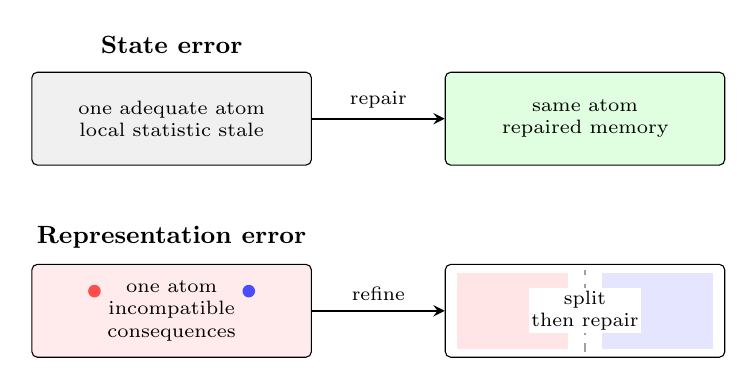
\begin{tikzpicture}[x=1cm,y=1cm,>=stealth]
\tikzset{
    panel/.style={draw,rounded corners=2pt,minimum width=3.55cm,minimum height=1.18cm,align=center,font=\scriptsize,text width=3.05cm},
    title/.style={font=\small\bfseries},
    flow/.style={->,thick}
}
\node[title] at (1.8,1.65) {State error};
\node[panel,fill=gray!12] (state0) at (1.8,0.72) {one adequate atom\\local statistic stale};
\node[panel,fill=green!12] (state1) at (7.05,0.72) {same atom\\repaired memory};
\draw[flow] (state0.east) -- node[above,font=\scriptsize] {repair} (state1.west);

\node[title] at (1.8,-0.78) {Representation error};
\node[panel,fill=red!8] (repr0) at (1.8,-1.72) {one atom\\incompatible consequences};
\fill[red!70] (0.82,-1.47) circle (0.08);
\fill[blue!70] (2.78,-1.47) circle (0.08);
\node[panel,fill=white] (repr1) at (7.05,-1.72) {};
\fill[red!10] (5.42,-2.20) rectangle (6.83,-1.24);
\fill[blue!10] (7.27,-2.20) rectangle (8.68,-1.24);
\draw[dashed,gray!75] (7.05,-2.24) -- (7.05,-1.96);
\draw[dashed,gray!75] (7.05,-1.48) -- (7.05,-1.20);
\node[font=\scriptsize,align=center,fill=white,inner sep=1pt] at (7.05,-1.72) {split\\then repair};
\draw[flow] (repr0.east) -- node[above,font=\scriptsize] {refine} (repr1.west);
\end{tikzpicture}
\caption{Runtime learning has two failure modes. Stale state should be repaired inside an adequate concept; incompatible consequences inside one atom require refinement.}
\label{fig:two-failure-modes}
\end{figure}

Many runtime-learning mechanisms implement one dominant response to surprise. Cache and $k$NN language models store or retrieve more examples \citep{grave2017improving,khandelwal2020generalization}. Fast weights and delta-rule linear attention repair associative state \citep{ba2016using,schlag2021linear}. Test-time training and adaptation optimize an inference-time surrogate \citep{sun2020test,wang2021tent,sun2025learning}. Online trees refine leaves by split scores \citep{breiman1984classification,domingos2000mining}. Sparse MoE routes to trained experts \citep{shazeer2017outrageously,fedus2022switch}. Adaptive category and prototype systems, including ART 1 and ART 2, create or move categories \citep{carpenter1987massively,carpenter1987art2,kohonen1990self,fritzke1995growing,snell2017prototypical}. DGM is not a claim that these ingredients are new. The claim is that a runtime learner should first decide which operation is legal: repair within the current information, or refine the information itself.

\begin{table}[t]
\centering
\small
\begin{tabular}{p{0.20\linewidth}p{0.31\linewidth}p{0.39\linewidth}}
\toprule
Method family & What it does when surprised & Why that is incomplete \\
\midrule
Cache/$k$NN-LM & store or retrieve more examples & does not decide whether a new concept is needed \\
Fast weights / local memories & repair associative state & cannot fix missing distinctions \\
TTT/TTA & optimize a test-time objective & treats adaptation as surrogate-loss descent \\
Online trees & split leaves & rooted hierarchy; no local repair memory at graph concepts \\
MoE / PKM & route to trained capacity & experts or keys are static, not runtime-created concepts \\
ART systems / prototypes & create or move categories & lacks edge-generated local repair structure \\
\bottomrule
\end{tabular}
\vspace{0.35em}
\begin{minipage}{0.96\linewidth}
\footnotesize
\emph{Representative references.}
Cache and $k$NN-LM: \citep{grave2017improving,khandelwal2020generalization};
fast weights and local memories: \citep{ba2016using,schlag2021linear};
TTT/TTA: \citep{sun2020test,wang2021tent,sun2025learning};
online trees: \citep{breiman1984classification,domingos2000mining};
MoE and PKM: \citep{shazeer2017outrageously,fedus2022switch,lample2019large};
ART, ART 2, and prototypes: \citep{carpenter1987massively,carpenter1987art2,kohonen1990self,fritzke1995growing,snell2017prototypical}.
\end{minipage}
\caption{Representative runtime-learning mechanisms and the single dominant update they apply when surprised. DGM's claim is not that these mechanisms are absent from prior work, but that runtime learning needs an explicit decision between refining the information structure and repairing state inside it.}
\label{tab:runtime-learning-comparison}
\end{table}

The separation is structural. A learner's information state can be represented by a partition or sigma-algebra, and its admissible predictors are precisely the measurable functions with respect to that information. If two states lie in the same atom but require different outputs, no predictor over the current information can satisfy both. More computation inside the atom cannot remove the contradiction. This is the paper's central diagnosis: a contradiction inside an atom is not a failed optimization step; it is a certificate that the atom is too coarse.

The formal core is then minimal information refinement. In a finite space, adding a binary distinction cuts exactly the old atoms crossed by that distinction and leaves all other atoms unchanged. In a general measurable space, the same operation is the join
\begin{align*}
\calF_{t+1}=\calF_t\vee\sigma(Z_t).
\end{align*}
This is the smallest information update that makes the new evidence observable, using standard language from measure-theoretic probability and statistical decision theory \citep{billingsley1995probability,kallenberg2002foundations,blackwell1953equivalent,berger1985statistical}. The value of the update is also exact: under log loss, refinement value is conditional mutual information; under squared loss, it is conditional variance reduction. Population information cannot hurt, but finite-sample estimation can. Thus a useful runtime learner should refine only when a statistically guarded gain test justifies the new distinction.

Distinction Graph Machines implement this theorem-to-algorithm path as a data structure. If contradictions require distinctions, the learner needs runtime concepts. If concepts must remain stable, each concept needs a frozen anchor. If retrieval must adapt, each concept also needs a movable centroid. If distinctions are local, the structure should add pairwise graph edges rather than rewrite a global tree. If concepts have state, each node should carry a repairable memory. A DGM therefore maintains anchored concepts, movable retrieval centroids, local memories, and distinction edges. Edges are not metadata: they are binary generators that define observable distinctions and gate future routing. When a consequence arrives, DGM either repairs local memory under fixed anchors and edges, or creates a new anchored concept and edges after a guarded refinement test.

\paragraph{Terminology.}
Throughout the paper, \emph{DGM} denotes the runtime machine as a whole. A \emph{concept} is a graph node. Each concept has a frozen \emph{anchor} $a_j$, a movable \emph{centroid} $c_j$, and a repairable \emph{memory} $M_j$. A \emph{distinction edge} is a binary generator stored between concepts. We use \emph{hard route} for the exact anchor-defined selector used in the theory, and \emph{soft read} for the differentiable edge-gated implementation. We reserve \emph{prototype} mostly for related work and for standard nearest-prototype terminology.

At one timestep, the whole mechanism has the structure in Algorithm~\ref{alg:refine-repair-template}.
\begin{algorithm}[H]
\caption{\textsc{RefineOrRepairStep} (structural template)}
\label{alg:refine-repair-template}
\begin{algorithmic}[1]
\State \textbf{Input:} runtime state and current context
\State \textbf{Read:} use the current concepts, edges, and memories to predict
\State \textbf{Observe:} receive the consequence for this context
\If{the current concept is adequate}
    \State \textbf{Repair:} update local state while keeping anchors and edges fixed
\Else
    \State \textbf{Refine:} add a concept and distinction edges, then initialize local state
\EndIf
\State \Return updated runtime state
\end{algorithmic}
\end{algorithm}
The template deliberately omits retrieval rules, edge gates, scoring buffers, and memory forms. The algorithms in Section~\ref{sec:algorithms} fill in those choices. The theory supplies the two tests behind the template: the contradiction theorem says when repair is impossible under the current information, and the value identities plus sample-split guard say when a proposed distinction is worth paying for. Thus DGM is not a generic memory with a growth heuristic; it is a runtime implementation of a decision-theoretic question: is the error measurable under the current information?

For language models, the canonical layer is DGM-Embedding. Hidden-state concepts store next-token embedding memories and produce sparse logit corrections. The read path is differentiable, so slow model parameters can learn to use DGM memory. The write path is detached and forward-only: after observing the next token, the layer repairs selected local memories or refines the concept graph without inference-time backpropagation. Projection Memory and Conservative Projection Memory (CPM) appear as local repair mechanisms once the relevant distinction structure has been fixed.

\paragraph{Contributions.}
The contribution is a separation theorem and its algorithmic realization.
\begin{itemize}
    \item \textbf{Obstruction.} We prove that some runtime errors are structurally unrepairable: if incompatible consequences lie inside one atom of the current information structure, no measurable predictor can satisfy them.
    \item \textbf{Canonical update.} We identify minimal refinement as the least information update that makes new evidence observable, and we quantify refinement value under log and squared losses.
    \item \textbf{Runtime machine.} We introduce DGM, a graph-based learner whose edges generate distinctions, whose anchors stabilize those distinctions, and whose local memories support guarded repair.
    \item \textbf{Language-model layer.} We instantiate DGM as DGM-Embedding, with differentiable sparse reads, detached forward-only writes, and an explicit bridge to projection-style repair.
\end{itemize}

\paragraph{Scope of the formal claims.}
The theorem-level question is not whether DGM is the globally optimal runtime architecture. It is: given a current information structure $\calF$, when is an error impossible to fix by any $\calF$-measurable repair, and what is the least information that must be added once a new distinction is required? Sections~\ref{sec:preliminaries}--\ref{sec:value} answer this question at the population level, and Section~\ref{sec:algorithms} gives finite-sample guarded versions for a finite candidate class. DGM and DGM-Embedding are algorithmic realizations of this refine-or-repair principle; optimization guarantees for deep nonconvex backbones and global search over all possible distinctions are outside the theorem statements.

\paragraph{Organization.}
Sections~\ref{sec:preliminaries}--\ref{sec:value} give the information-structure obstruction, the minimal refinement rule, and the value identities. Section~\ref{sec:algorithms} turns the theory into Distinction Graph Machines. Section~\ref{sec:large-model-training} gives DGM-Embedding for language models. Section~\ref{sec:technical-overview} summarizes the guarantees, Section~\ref{sec:projection-bridge} relates the repair side to Projection Memory and CPM, and Section~\ref{sec:experiments} gives computational checks.

\section{Repair and Refinement Gaps}
\label{sec:preliminaries}

The main theory diagnoses which part of a runtime error is being observed. The representation map $I_t$ determines the information $\calF_t=\sigma(I_t)$ available to the learner. The predictor $f_t$ is the current decision rule. A candidate refinement $\calG\supseteq\calF_t$ is a richer information structure. The two gaps $\Delta_{\mathrm{repair}}$ and $\Delta_{\mathrm{refine}}$ compare these three objects.

\paragraph{Notation.}

All probability spaces are denoted by $(\Omega,\calE,\mathbb P)$ unless the finite case is stated explicitly. Every information structure, including $\calF_t$ and $\calG$, is a sub-sigma-algebra of $\calE$. Random variables are functions on $\Omega$. We reserve $\mathsf A$ for the action space, $I_t$ for the information map, $\calZ_t$ for its label space, $Y$ for the consequence to be predicted, and $U_t$ for newly observed evidence used in a refinement. For a sub-sigma-algebra $\calF$, define
\begin{align*}
\Pred(\calF)=\{a:\Omega\to\mathsf A: a\text{ is }\calF\text{-measurable}\}.
\end{align*}
In the DGM sections, $E_t$ or $E(\calS)$ denotes a graph edge set, $\operatorname{Inc}_t(j)$ denotes the edges incident to concept $j$, and $e_y$ denotes the output embedding of label $y$. We use standard measure-theoretic probability notation for generated sigma-algebras, joins, measurability, and conditional expectation \citep{billingsley1995probability,kallenberg2002foundations}. For vectors $x\in\R^d$, lengths use the $\ell_2$ norm $\norm{x}_2$. For matrices, $\norm{M}_F$ is the Frobenius norm. Inner products are written $\ip{x}{y}$.

\subsection{Information maps and fibers}

At time $t$, let
\begin{align*}
I_t:\Omega\to\calZ_t
\end{align*}
be the learner's current information map. The value $I_t(\omega)$ is the runtime state label available to the learner. Two worlds $\omega,\omega'$ are indistinguishable under the current representation when $I_t(\omega)=I_t(\omega')$. The fiber, or cell,
\begin{align*}
I_t^{-1}(z)=\{\omega:I_t(\omega)=z\}
\end{align*}
is the set of worlds currently treated as the same situation. The sigma-algebra generated by the current information is
\begin{align*}
\calF_t=\sigma(I_t).
\end{align*}

In the finite setting, this is equivalent to a partition
\begin{align*}
\calP=\{B_1,\ldots,B_n\}
\end{align*}
of $\Omega$ into nonempty disjoint cells. A partition $\calQ$ refines $\calP$ if every cell of $\calQ$ is contained in a cell of $\calP$. An event $D\subseteq\Omega$ is $\calP$-measurable if it is a union of cells of $\calP$. Thus a partition is not only notation. It is the learner's current quotient of the world into distinguishable cases.

For sigma-algebras $\calF,\calG\subseteq\calE$, the inclusion $\calF\subseteq\calG$ means that $\calG$ is at least as informative as $\calF$. The join $\calF\vee\calG$ is the smallest sigma-algebra containing both. For a random variable $U$, $\sigma(U)$ is the sigma-algebra generated by $U$; for an event $D$, $\sigma(D)=\{\varnothing,D,D^c,\Omega\}$.

\subsection{Measurable predictors}

A measurable predictor is what the learner is allowed to compute from its current distinctions. With information map $I_t$, the runtime predictor has the form
\begin{align*}
f_t(\omega)=g_t(I_t(\omega))
\end{align*}
for some downstream rule $g_t$. Equivalently, $f_t$ is $\calF_t$-measurable. In a finite partition, a prediction or action $f:\Omega\to\mathsf A$ is $\calP$-measurable if it is constant on each cell:
\begin{align*}
\omega,\omega'\in B\in\calP\quad \Longrightarrow\quad f(\omega)=f(\omega').
\end{align*}
Equivalently, $f$ can depend only on the cell containing the current world state. In the sigma-algebra setting, the admissible predictors are exactly $\Pred(\calF)$. This is the formal reason a missing distinction cannot be repaired by a more clever local update inside the same cell: the update still returns a function on the same quotient.

\subsection{Bayes risk under information}

Bayes risk under information is the best possible performance given the distinctions currently available. Let $Y:\Omega\to\calY$ be a target random variable and let $L:\calY\times\mathsf A\to\R$ be a loss for which the expectations below are well-defined. The Bayes risk available under information $\calF$ is
\begin{align}
R_L(\calF)=\inf_{a\in\Pred(\calF)}\E[L(Y,a)].
\label{eq:bayes-risk}
\end{align}
Thus $R_L(\calF)$ is the best population risk achievable by a predictor that can use only distinctions in $\calF$, following the standard decision-theoretic view of actions, losses, Bayes risk, and comparison of information structures \citep{blackwell1953equivalent,berger1985statistical}.

\subsection{Repair and refinement}

For a concrete predictor $f$, write its risk as
\begin{align*}
R_L(f)=\E[L(Y,f)].
\end{align*}
A \emph{repair} update preserves information:
\begin{align*}
\calF_{t+1}=\calF_t.
\end{align*}
At the population level, a repair can only move within the class of $\calF_t$-measurable predictors, whose optimal risk is $R_L(\calF_t)$. The corresponding repair gap is
\begin{align}
\Delta_{\mathrm{repair}}(f_t,\calF_t)
=
R_L(f_t)-R_L(\calF_t).
\label{eq:repair-gap}
\end{align}

A \emph{refinement} update changes information:
\begin{align*}
\calG\supsetneq\calF_t.
\end{align*}
For a candidate refinement $\calG$, the refinement gap is
\begin{align}
\Delta_{\mathrm{refine}}(\calF_t,\calG)
=
R_L(\calF_t)-R_L(\calG).
\label{eq:refinement-gap}
\end{align}
We omit the loss $L$ from the $\Delta$ notation because the surrounding risk functional already fixes it. The quantity $\Delta_{\mathrm{repair}}$ is residual error under the current information. The quantity $\Delta_{\mathrm{refine}}$ is the value of distinctions not yet present in the current information.

\begin{theorem}[Runtime error decomposition]
\label{thm:error-decomposition}
Let $f_t$ be $\calF_t$-measurable and let $\calG\supseteq\calF_t$ be a candidate refinement. Then
\begin{align}
R_L(f_t)-R_L(\calG)
=
\Delta_{\mathrm{repair}}(f_t,\calF_t)
+
\Delta_{\mathrm{refine}}(\calF_t,\calG).
\label{eq:error-decomposition}
\end{align}
Both terms are nonnegative.
\end{theorem}

\begin{proof}
Add and subtract $R_L(\calF_t)$. The term $\Delta_{\mathrm{repair}}$ is nonnegative because $R_L(\calF_t)$ is the infimum over all $\calF_t$-measurable predictors, including $f_t$. The term $\Delta_{\mathrm{refine}}$ is nonnegative because every $\calF_t$-measurable predictor is also $\calG$-measurable when $\calF_t\subseteq\calG$.
\end{proof}

\subsection{Contradiction inside a cell}

The hard-label obstruction is the clearest special case of positive $\Delta_{\mathrm{refine}}$. If a cell contains states that require different outputs, the current information structure does not merely have a bad parameter value; it lacks the expressive degree of freedom needed to represent the target.

\begin{corollary}[Contradiction requires distinction]
\label{thm:contradiction:informal}
Let $I:\Omega\to\calZ$ be an information map and let $y:\Omega\to\mathsf A$ be a required output. Suppose $I(\omega)=I(\omega')$ but $y(\omega)\ne y(\omega')$. Then no predictor of the form $f=g\circ I$ satisfies both $f(\omega)=y(\omega)$ and $f(\omega')=y(\omega')$.
\end{corollary}

\begin{proof}
If $f=g\circ I$ and $I(\omega)=I(\omega')$, then $f(\omega)=f(\omega')$. Satisfying both required outputs would imply $y(\omega)=y(\omega')$, a contradiction.
\end{proof}

This corollary is deliberately architecture-independent. It applies to a neural cache, a local adapter, a fast-weight memory, a nearest-neighbor system, or a test-time optimizer whenever the update is constrained to the current information. If the relevant states are not separated by $I$, no repair rule inside the cell can represent the required behavior. The contradiction is evidence that the cell should be split.

\begin{example}[One prefix, two consequences]
Suppose the current runtime concept groups two prefixes because their surface form is the same. In one hidden regime the next token should be ``red''; in another it should be ``blue''. Any memory attached to the single concept must store one consequence distribution for both regimes. A repair update can move that distribution, but it cannot make it simultaneously put all mass on ``red'' and all mass on ``blue''. The missing operation is to split the concept by a distinction correlated with the hidden regime, then repair the two resulting memories separately.
\end{example}

\subsection{Minimal refinement}
\label{sec:minimal-refinement}

Once a contradiction shows that the current atom is too coarse, the next question is not how to grow a large model. It is which information must be added. The primitive operation in this paper is minimal refinement: given an information structure and evidence that a new event or variable must be observable, add that observability and nothing else. We state the finite partition theorem first, then the sigma-algebra form. The latter is the standard measure-theoretic join; the former is its finite special case \citep{billingsley1995probability,kallenberg2002foundations}.

\subsubsection{The finite refinement rule}

Let $\calP$ be a finite partition and let $D\subseteq\Omega$ be a new binary distinction event. Define
\begin{align}
\calP_D
&=\{B\cap D:B\in\calP, B\cap D\ne\varnothing\}\notag\\
&{}\cup\{B\cap D^c:B\in\calP, B\cap D^c\ne\varnothing\}.
\label{eq:finite-refinement}
\end{align}
This keeps exactly the nonempty pieces obtained by cutting each old atom by $D$.

\begin{theorem}[Minimal finite refinement]
\label{thm:minimal-refinement:informal}
Let $\calP$ be a finite partition of $\Omega$ and let $D\subseteq\Omega$. The partition $\calP_D$ is the unique minimal partition that refines $\calP$ and makes $D$ measurable. More precisely, if $\calQ$ refines $\calP$ and $D$ is $\calQ$-measurable, then $\calQ$ refines $\calP_D$.
\end{theorem}

\begin{proof}
Each old atom $B\in\calP$ is replaced by the nonempty sets among $B\cap D$ and $B\cap D^c$, so the resulting sets are disjoint, cover $\Omega$, and each lies inside an atom of $\calP$. Hence $\calP_D$ is a refinement of $\calP$. Moreover,
\begin{align*}
D=\bigcup_{B\in\calP}(B\cap D),
\end{align*}
so $D$ is a union of $\calP_D$-atoms. Now let $\calQ$ refine $\calP$ and make $D$ measurable. For every $Q\in\calQ$, there is $B\in\calP$ with $Q\subseteq B$, and measurability of $D$ with respect to $\calQ$ implies either $Q\subseteq D$ or $Q\subseteq D^c$. Thus $Q$ is contained in either $B\cap D$ or $B\cap D^c$, i.e., in an atom of $\calP_D$. Therefore $\calQ$ refines $\calP_D$.
\end{proof}

The theorem gives a canonical update. The evidence determines the least refined representation: atoms untouched by $D$ remain unchanged, while atoms crossed by $D$ split into the two pieces that the evidence distinguishes.

\subsubsection{The sigma-algebra form}

For general spaces, the same operation is the join of sigma-algebras. If the current information is $\calF_t$ and the evidence is a variable $U_t$, the minimal updated information is
\begin{align}
\calF_{t+1}=\calF_t\vee\sigma(U_t).
\label{eq:join-update}
\end{align}

\begin{theorem}[Minimal sigma-algebra refinement]
\label{thm:sigma-refinement:informal}
Let $\calF\subseteq\calE$ be a sigma-algebra and let $U$ be a random variable. The join $\calF\vee\sigma(U)$ is the smallest sigma-algebra $\calG$ such that $\calF\subseteq\calG$ and $U$ is $\calG$-measurable.
\end{theorem}

\begin{proof}
By definition, $\calF\vee\sigma(U)=\sigma(\calF\cup\sigma(U))$, so it contains $\calF$ and makes $U$ measurable. If another sigma-algebra $\calG$ contains $\calF$ and makes $U$ measurable, then $\calF\cup\sigma(U)\subseteq\calG$. Since $\calG$ is a sigma-algebra, $\sigma(\calF\cup\sigma(U))\subseteq\calG$.
\end{proof}

Thus the same object governs finite decision-tree splits and measurable-space refinement. A distinction is not an auxiliary feature added after learning; it is a change in the sigma-algebra of what the learner may condition on. The obstruction in Section~\ref{sec:preliminaries} says when such a change is necessary; minimal refinement says how little information must be added.

\section{The Value of a Distinction}
\label{sec:value}

Minimal refinement says how to add a distinction; it does not license every possible distinction. The value question is task-dependent: when does the new distinction actually change the best achievable prediction? We measure this by the decrease in optimal risk after the information structure is refined, in the same decision-theoretic sense used in classical comparisons of statistical experiments and value of information \citep{blackwell1953equivalent,berger1985statistical}.

\subsection{Risk monotonicity}

The first fact is purely order-theoretic. If $\calG$ contains all events in $\calF$, then every $\calF$-measurable predictor is also $\calG$-measurable. The decision class has only grown; this is the Bayes-risk analogue of Blackwell's monotonicity of decision value under more informative experiments \citep{blackwell1953equivalent}.

\begin{theorem}[Bayes-risk monotonicity]
\label{thm:risk-monotonicity:informal}
If $\calF\subseteq\calG$, then for every loss $L$ for which both risks are well-defined,
\begin{align*}
R_L(\calG)\le R_L(\calF).
\end{align*}
\end{theorem}

This is a population statement. It says that information cannot hurt the best possible decision rule. It does not say that a finite implementation should refine without restraint. Statistical estimation, finite samples, and model selection can overfit; those are algorithmic questions, not failures of the information order. This is why the DGM algorithm later uses penalties, thresholds, and sample-split scoring before committing a new concept.

\subsection{Log loss}

For a finite target variable $Y$, log loss asks the learner to output a conditional distribution. The optimal prediction under $\calF$ is the conditional law of $Y$ given $\calF$, and the optimal risk is conditional entropy, a standard identity for logarithmic scoring rules and information theory \citep{cover2006elements,gneiting2007strictly}.

\begin{theorem}[Log-loss value]
\label{thm:log-value:informal}
Let $Y$ be finite and let the loss be $-\log q(Y)$. If $\calF\subseteq\calG$, then
\begin{align*}
R_{\log}(\calF)-R_{\log}(\calG)=I(Y;\calG\mid\calF).
\end{align*}
\end{theorem}

Here $I(Y;\calG\mid\calF)$ denotes $H(Y\mid\calF)-H(Y\mid\calG)$. Thus, for classification and language modeling, a refinement is useful exactly to the extent that it carries conditional mutual information about the consequence beyond what the learner already knows. If the new bit does not tell us anything about the next consequence beyond the old information, it is a gratuitous distinction, even if it separates inputs.

\subsection{Squared loss}

For $Y\in L^2(\Omega;\R^d)$ and squared loss, the optimal predictor under $\calF$ is $\E[Y\mid\calF]$, the $L^2$ projection onto the closed subspace of $\calF$-measurable random variables \citep{billingsley1995probability,kallenberg2002foundations}. Refinement helps precisely when it changes the conditional mean.

\begin{theorem}[Squared-loss value]
\label{thm:squared-value:informal}
Let $Y\in L^2(\Omega;\R^d)$ and let $L(Y,a)=\norm{Y-a}_2^2$. If $\calF\subseteq\calG$, then
\begin{align*}
R_2(\calF)-R_2(\calG)=\E\left[\norm{\E[Y\mid\calG]-\E[Y\mid\calF]}_2^2\right].
\end{align*}
\end{theorem}

The identity is the Hilbert-space analogue of the log-loss result. A distinction has squared-loss value when the cells it creates have different conditional means. In regression language, refinement is worth paying for when it separates consequences, not merely when it separates inputs.

\subsection{Finite empirical scores}

The population identities lead directly to standard empirical split scores: information gain for classification and variance reduction for regression trees \citep{breiman1984classification,domingos2000mining}. Suppose an atom $B$ contains samples $(x_j,y_j)$ and a candidate distinction $g:B\to\{0,1\}$ splits it into $B_0$ and $B_1$.

For classification, let $\hat p_B$, $\hat p_{B_0}$, and $\hat p_{B_1}$ be empirical label distributions. The empirical log-loss improvement is
\begin{align*}
\Delta_{\log}(B,g)=\abs{B}H(\hat p_B)-\abs{B_0}H(\hat p_{B_0})-\abs{B_1}H(\hat p_{B_1}).
\end{align*}
Equivalently,
\begin{align*}
\Delta_{\log}(B,g)=\abs{B}\widehat I(Y;g\mid B).
\end{align*}

For regression, define
\begin{align*}
\hat\mu_B=\frac{1}{\abs{B}}\sum_{j\in B}y_j,\qquad \operatorname{SSE}(B)=\sum_{j\in B}\norm{y_j-\hat\mu_B}_2^2.
\end{align*}
The empirical squared-loss improvement is
\begin{align*}
\Delta_2(B,g)=\operatorname{SSE}(B)-\operatorname{SSE}(B_0)-\operatorname{SSE}(B_1).
\end{align*}
It also has the between-cell form
\begin{align*}
\Delta_2(B,g)=\abs{B_0}\norm{\hat\mu_{B_0}-\hat\mu_B}_2^2+\abs{B_1}\norm{\hat\mu_{B_1}-\hat\mu_B}_2^2.
\end{align*}

These scores implement the same principle as the population theory: split only when the proposed distinction has measurable consequence value. The DGM algorithm below turns this population rule into a guarded empirical decision.

\section{Distinction Graph Machines}
\label{sec:algorithms}

The tree model is a useful finite special case, but it is not the most natural runtime data structure. A tree makes every decision through one irreversible path. A more flexible object is a graph of concepts: local memories live at prototypes, and distinctions live on edges between prototypes that have been confused. This section defines that model.

\subsection{State and prediction}

Let $\phi_\theta:\calX\to\R^d$ be an encoder. A Distinction Graph Machine has runtime state
\begin{align*}
\calS_t=\left(\{c_j,M_j,n_j\}_{j=1}^{N_t},G_t\right).
\end{align*}
Here $c_j\in\R^d$ is a prototype, $M_j$ is a local predictor or memory, $n_j$ is a usage count, and $G_t$ is a graph on the prototypes. An edge $(i,j)$ stores a distinction separating the two concepts, typically
\begin{align*}
u_{ij}=\frac{c_i-c_j}{\norm{c_i-c_j}_2},\qquad b_{ij}=\frac{1}{2}u_{ij}^\top(c_i+c_j).
\end{align*}
The edge distinction is
\begin{align*}
g_{ij}(h)=\one\{u_{ij}^\top h>b_{ij}\}.
\end{align*}

Given $h=\phi_\theta(x)$, the machine computes distances $d_j(h)$ to prototypes and a sparse neighborhood
\begin{align*}
N_k(h)\subseteq\{1,\ldots,N_t\}.
\end{align*}
It then forms routing weights
\begin{align*}
\alpha_j(h)=\frac{\exp(-d_j(h)/T)}{\sum_{r\in N_k(h)}\exp(-d_r(h)/T)}
\qquad j\in N_k(h),
\end{align*}
and predicts by local mixture
\begin{align*}
\hat y=\sum_{j\in N_k(h)}\alpha_j(h)M_j(h).
\end{align*}
Hard nearest-prototype routing is the limit $T\to0$.

\begin{algorithm}[H]
\caption{\textsc{Predict} for a Distinction Graph Machine}
\label{alg:dgm-predict}
\begin{algorithmic}[1]
\State \textbf{Input:} state $\calS_t=(\{c_j,M_j,n_j\}_{j=1}^{N_t},G_t)$, encoder $\phi_\theta$, example $x$
\State $h\gets\phi_\theta(x)$
\State $N_k(h)\gets$ the $k$ nearest prototypes to $h$
\State compute weights $\alpha_j(h)$ for $j\in N_k(h)$
\State \Return $\sum_{j\in N_k(h)}\alpha_j(h)M_j(h)$
\end{algorithmic}
\end{algorithm}

\subsection{Refine or repair on a graph}

After observing consequence $y$, DGM first asks whether an existing concept can absorb the evidence. Let $j^\star$ be the nearest or highest-weight prototype. Define a local inconsistency score
\begin{align*}
\rho_t=L(y,M_{j^\star}(h)).
\end{align*}
If $\rho_t$ is small, the information structure is treated as adequate and the machine repairs the local state:
\begin{align*}
M_{j^\star}\leftarrow\operatorname{Repair}(M_{j^\star},h,y),
\qquad
c_{j^\star}\leftarrow c_{j^\star}+\eta_c(h-c_{j^\star}),
\qquad
n_{j^\star}\leftarrow n_{j^\star}+1.
\end{align*}
If $\rho_t$ is large and the neighborhood contains incompatible consequences, the machine refines by creating a new prototype
\begin{align*}
c_{N_t+1}=h,\qquad M_{N_t+1}=\operatorname{InitMemory}(h,y),
\end{align*}
and adds distinction edges from the new prototype to the confused neighbors.

\begin{algorithm}[H]
\caption{\textsc{Observe} for a Distinction Graph Machine}
\label{alg:dgm-observe}
\begin{algorithmic}[1]
\State \textbf{Input:} state $\calS_t$, labeled consequence $(x,y)$
\State $h\gets\phi_\theta(x)$
\If{$N_t=0$}
\State create prototype $c_1=h$ with memory $\operatorname{InitMemory}(h,y)$
\State \Return updated state
\EndIf
\State $j^\star\gets\argmin_j d_j(h)$
\State $\rho\gets L(y,M_{j^\star}(h))$
\If{$\rho\le\tau_{\mathrm{repair}}$}
\State repair $M_{j^\star}$ and move $c_{j^\star}$ toward $h$
\Else
\State create a new prototype $c_{N_t+1}=h$
\State initialize $M_{N_t+1}$ from $(h,y)$
\For{confused neighbor $i$ of $h$}
\State add edge $(i,N_t+1)$ with distinction $(u_{i,N_t+1},b_{i,N_t+1})$
\EndFor
\EndIf
\State \Return updated state
\end{algorithmic}
\end{algorithm}

\begin{theorem}[Prototype distinction separates its endpoints, informal version of Theorem~\ref{thm:prototype-edge:formal}]
\label{thm:prototype-edge:informal}
If $c_i\ne c_j$ and $u_{ij},b_{ij}$ are defined as above, then
\begin{align*}
u_{ij}^\top c_i-b_{ij}=\frac{1}{2}\norm{c_i-c_j}_2,
\qquad
u_{ij}^\top c_j-b_{ij}=-\frac{1}{2}\norm{c_i-c_j}_2.
\end{align*}
Thus each edge distinction separates the two prototypes that caused it.
\end{theorem}

\subsection{Why graph memory is different from a tree}

A tree stores distinctions as a hierarchy. A mistake near the root changes every downstream routing decision. A graph stores distinctions locally between concepts. Creating a new concept does not rewrite old paths; it adds a local alternative and edges explaining why the new concept differs from its neighbors.

A binary distinction tree is recovered by restricting $G_t$ to a rooted binary hierarchy and forcing every input to follow a single path. DGM is therefore the parent data structure; trees are a sparse, hard-routing special case.

\subsection{Local memories}

The local memory $M_j$ can be chosen according to the task.

\begin{itemize}
\item {\bf Classification.} $M_j$ stores label counts or exemplars associated with prototype $j$.
\item {\bf Regression.} $M_j$ stores a local mean, local linear model, or ridge regressor.
\item {\bf Associative repair.} $M_j$ stores a Projection Memory matrix $W_j$ and updates it by
\begin{align*}
W_{j,t+1}=W_{j,t}+\frac{\eta}{1+\eta\norm{k_t}_2^2}(v_t-W_{j,t}k_t)k_t^\top.
\end{align*}
\end{itemize}

The conceptual rule is unchanged: if the prototype is adequate, repair its local state; if evidence is incompatible with the current prototypes, create a new distinction.

\subsection{Language modeling instance}
\label{sec:language-dgm}

For language modeling, the world state is a prefix and the consequence is the next observed token. Let a frozen or slowly trained backbone produce hidden states
\begin{align*}
h_t=\phi_\theta(x_{\le t}).
\end{align*}
DGM is inserted as a runtime memory over hidden states. Each prototype $c_j$ represents a recurring context type: a citation pattern, a local syntax regime, a document-specific entity usage, or a repeated task format. The local memory $M_j$ predicts a correction to the next-token distribution.

A scalable instance stores a target embedding mean
\begin{align*}
r_j=\frac{1}{n_j}\sum_{s\in C_j}E[x_{s+1}],
\end{align*}
where $E[y]\in\R^{d_e}$ is the output embedding of token $y$. For a new prefix, DGM retrieves prototypes $N_k(h_t)$ and forms the correction
\begin{align*}
\ell_{\mathrm{DGM}}(y\mid h_t)=\sum_{j\in N_k(h_t)}\alpha_j(h_t)E[y]^\top r_j.
\end{align*}
The final logits are
\begin{align*}
\ell(y\mid x_{\le t})=\ell_\theta(y\mid x_{\le t})+\lambda_t\ell_{\mathrm{DGM}}(y\mid h_t).
\end{align*}
Here $\lambda_t$ is a learned or fixed trust weight. After the next token $x_{t+1}$ is observed, the machine updates by \textsc{Observe} with consequence $y=x_{t+1}$. If an existing prototype is repaired, its embedding memory can be updated by
\begin{align*}
r_j^+=\frac{n_jr_j+E[x_{t+1}]}{n_j+1},
\qquad
n_j^+=n_j+1.
\end{align*}
If the observed next token is surprising under the nearest prototype and the context is not well explained by existing prototypes, DGM creates a new prototype at $h_t$ and initializes
\begin{align*}
c_{N_t+1}=h_t,
\qquad
r_{N_t+1}=E[x_{t+1}],
\qquad
n_{N_t+1}=1.
\end{align*}

This gives a direct test-time learning protocol for language modeling. During streaming prediction, document continuation, user correction, tool feedback, or supervised next-token evaluation, the next observed token is genuine evidence and can refine or repair the runtime memory. During unconstrained generation, the model should not update from its own sampled token by default, because self-generated samples are actions, not external consequences.

\begin{algorithm}[H]
\caption{\textsc{ObserveNextToken} for DGM language modeling}
\label{alg:dgm-lm}
\begin{algorithmic}[1]
\State \textbf{Input:} prefix $x_{\le t}$, observed token $x_{t+1}$, DGM state $\calS_t$
\State $h_t\gets\phi_\theta(x_{\le t})$
\State retrieve $N_k(h_t)$ and compute logits $\ell_\theta+\lambda_t\ell_{\mathrm{DGM}}$
\State $j^\star\gets$ nearest or highest-weight prototype
\State $\rho\gets-\log p(x_{t+1}\mid x_{\le t})$
\If{$\rho\le\tau_{\mathrm{repair}}$}
\State update the local token memory at $j^\star$
\Else
\State create a new prototype at $h_t$ with local memory initialized by $E[x_{t+1}]$
\State add distinction edges to confused neighboring prototypes
\EndIf
\State \Return updated state
\end{algorithmic}
\end{algorithm}

\subsection{Complexity}

With exact nearest-neighbor search, prediction costs
\begin{align*}
O(N_td+kd+C_{\mathrm{local}}),
\end{align*}
where $C_{\mathrm{local}}$ is the cost of evaluating the selected local memories. With approximate nearest-neighbor indexing, the $N_td$ term can be replaced by the query cost of the index. Creating a prototype costs $O(d)$ plus the cost of initializing its memory. Adding $q$ distinction edges costs $O(qd)$. If each prototype stores an embedding mean in $\R^{d_e}$, runtime memory is
\begin{align*}
O(N_t(d+d_e)+|E_t|d).
\end{align*}

\begin{theorem}[DGM data-structure bound, informal version of Theorem~\ref{thm:dpm-complexity:formal}]
\label{thm:dpm-complexity:informal}
For exact search over $N_t$ prototypes in $\R^d$, one DGM prediction costs $O(N_td+kd+C_{\mathrm{local}})$. One observation that repairs a selected prototype costs this plus the local repair cost. One observation that creates a new prototype and $q$ distinction edges costs an additional $O(d+qd)$. With embedding-mean memories, the runtime state uses $O(N_t(d+d_e)+|E_t|d)$ memory.
\end{theorem}

\section{CoM: Concept Memory Language Modeling}
\label{sec:large-model-training}

For language modeling, the world state is a prefix and the consequence is the next token. Concept Memory (CoM) replaces the causal attention sublayer inside a decoder block with a concept-addressed memory update:
\begin{align*}
\operatorname{CABlock}(X)
=
X+\operatorname{CA}(\operatorname{Norm}(X)).
\end{align*}
The block has the same external shape contract as attention, $[B,L,d_{\rm model}]\mapsto[B,L,d_{\rm model}]$. The residual stream, layer normalization, embeddings, and language-model head are otherwise standard decoder components. In a Transformer-style decoder, CA can be paired with the usual MLP sublayer. For the state-matched PoST LM runs, the default implementation uses the same mixer-only residual scaffold as the Mamba-2 baseline; an MLP sublayer is an explicit configuration option rather than part of the main comparison.

\subsection{Fixed concept memory}

At layer $\ell$, CoM keeps a fixed bank of $C$ concept identities $a_{\ell hj}\in\mathbb{R}^{d_a}$ for each head $h$ and concept slot $j$. These identities are sequence-independent layer parameters, initialized as random unit vectors and trained by ordinary backpropagation. They are addresses shared across sequences, not online state. The online state is the value memory
\begin{align*}
M_t^\ell\in\mathbb{R}^{H\times C\times d_v^c}.
\end{align*}
Each token produces read queries, write keys, write values, and retention-decay projections:
\begin{align*}
q_t=Q_\ell x_t,\qquad k_t=K_\ell x_t,\qquad v_t=V_\ell x_t.
\end{align*}
The read is causal: token $t$ reads only concept values produced by earlier writes. For concept slots $j=1,\ldots,C$,
\begin{align*}
\alpha_{thj}
=
\operatorname{softmax}_{j}
\left(\gamma_\ell q_{th}^\top a_{\ell hj}\right),
\qquad
z_{th}=\sum_{j=1}^{C}\alpha_{thj}M_{t,hj}^\ell,
\qquad
y_t=O_\ell[z_{t1};\ldots;z_{tH}].
\end{align*}
Multi-head CA uses independent address and value subspaces per head and concatenates the head outputs before the output projection, exactly as multi-head attention does.

\subsection{Read before write}

The update order is the same during training and autoregressive inference:
\begin{align*}
\text{read from }M_t^\ell
\rightarrow
\text{emit }y_t
\rightarrow
\text{decay and write }(k_t,v_t)
\rightarrow
\text{update }M_{t+1}^\ell .
\end{align*}
This prevents a token from reading its own write. The inference-time update is the test-time learning mechanism in CoM: the model weights are fixed, but the concept value memory changes after the causal write and future tokens condition on that updated memory.

For a delayed write key $\bar k_t=k_{t-\delta}$, CA computes write weights
\begin{align*}
\beta_{thj}
=
\operatorname{softmax}_{j}
\left(\gamma_\ell \bar k_{th}^\top a_{\ell hj}\right).
\end{align*}
With retention factor $\rho_{th}$, the token-level streaming update is
\begin{align*}
M_{t+1,hj}^{\ell}
=
\rho_{th}M_{t,hj}^{\ell}
+\mathbf{1}_{t\ge\delta}\beta_{thj}v_{th}.
\end{align*}
For parallel training, CA groups tokens into chunks but keeps the same token-level recurrence. For chunk $b=[s,e)$, define the exact affine summary
\begin{align*}
U_{b,hj}^{\ell}
=
\sum_{t=s}^{e-1}
\left(\prod_{u=t+1}^{e-1}\rho_{uh}^{\ell}\right)
\mathbf{1}_{t\ge \delta}
\beta_{thj}v_{th},
\qquad
\rho_{bh}^{\ell}
=
\prod_{t=s}^{e-1}\rho_{th}^{\ell}.
\end{align*}
The chunk transition is
\begin{align*}
M_{e,hj}^{\ell}
=
\rho_{bh}^{\ell}M_{s,hj}^{\ell}
+U_{b,hj}^{\ell}.
\end{align*}
Thus each chunk is summarized by an affine map $(\rho_b,U_b)$. These summaries compose associatively:
\begin{align*}
(\rho_2,U_2)\odot(\rho_1,U_1)
=
(\rho_2\rho_1,\ U_2+\rho_2U_1),
\end{align*}
with identity $(1,0)$. The prefix memory before every chunk can therefore be recovered by an exclusive associative scan over the chunk summaries. After the scan, the implementation computes exact causal reads inside each chunk:
\begin{align*}
M_{t,hj}^{\ell}
=
\left(\prod_{u=s}^{t-1}\rho_{uh}^{\ell}\right)M_{s,hj}^{\ell}
+
\sum_{r=s}^{t-1}
\left(\prod_{u=r+1}^{t-1}\rho_{uh}^{\ell}\right)
\mathbf{1}_{r\ge\delta}\beta_{rhj}v_{rh}.
\end{align*}
Thus the chunked implementation is mathematically equivalent to the streaming read-before-write recurrence. The block size controls kernel tiling and scan granularity, not a different causal model.

The current fixed-bank CoM path writes every valid token with unit mass through the concept write distribution, while delayed-key runs use only the causal valid-write mask. The experiments use a trainable retention factor with a PoST-style ordered decay parameterization, input-dependent step sizes in a bounded range, and optional position-adaptive scaling. These are parameterization choices for stable allocation of forgetting time scales, not the definition of CA itself; CA can be run with a free retention parameterization for ablations.

\paragraph{First-principles update constraint.}
The state update must be more than a compressed token table. Under log loss, a useful runtime state is one that preserves or creates prediction-relevant distinctions in the prefix; a rule that only pools token values into slots can repair local averages, but it has no reason to form a local predictive model. The right test-time object is therefore a predictive statistic in concept coordinates: after observing a prefix event, the state should update the conditional predictor used by future concept queries, without running backpropagation at test time.

\paragraph{Gradient-free Concept Memory.}
Let $c_t\in\Delta^{C-1}$ be the concept responsibility of the context used to predict a consequence $Y_t$; in a language model, $Y_t$ is the next observed token or a learned consequence feature of that token. A concept-memory update is first-principled when it is the closed-form online estimator for the local prediction problem. For squared loss in a target feature space $u(Y_t)\in\mathbb{R}^{d_u}$, the sufficient statistics are discounted responsibility mass and first moment:
\begin{align*}
n_{t+1}
&=
\lambda_t n_t+c_t,
&
B_{t+1}
&=
\lambda_t B_t+c_t u(Y_t)^\top .
\end{align*}
The read used by a future query $q_t$ is the normalized conditional mean
\begin{align*}
z_t
=
q_t^\top
\left[
\operatorname{diag}(n_t+\alpha)^{-1}
\left(B_t+\alpha \mathbf{1}\mu_0^\top\right)
\right].
\end{align*}
This update is causal, online, and gradient-free. It is not a write gate: $c_t$ is the concept responsibility of the observed event, $n_t$ is the accumulated evidence for each concept, and the normalization prevents frequent concepts from merely accumulating larger vector norms.

For log loss with a finite vocabulary, the exact conjugate analogue is a concept-indexed categorical statistic
\begin{align*}
A_{t+1,jv}
=
\lambda_t A_{t,jv}+c_{tj}\mathbf{1}\{Y_t=v\},
\qquad
n_{t+1,j}
=
\lambda_t n_{tj}+c_{tj},
\end{align*}
and the fast prediction is
\begin{align*}
p_t(v)
=
\sum_{j=1}^{C}
q_{tj}
\frac{A_{t,jv}+\alpha p_0(v)}{n_{tj}+\alpha}.
\end{align*}
This is the Bayes-optimal repair inside a fixed concept partition for the multinomial-Dirichlet model. A full $C\times |V|$ table is usually too large, so the practical CoM form stores low-rank token features or residual logit factors instead of full vocabulary counts, but the statistical target is the same: the runtime state estimates a local conditional consequence distribution, not a hidden-value cache.

The scalable implementation chooses a consequence feature map
\begin{align*}
u(Y_t)=R e(Y_t)\in\mathbb{R}^{d_u},
\end{align*}
where $e(Y_t)$ is the output-embedding feature of the observed token and $R$ may be the identity or a fixed low-dimensional sketch. The fast state size is then $C(d_u+1)$ rather than $C(d_{\rm model}+1)$ or $C|V|$. This compression is not sparse retrieval: every concept can still be read and updated. It is the sufficient statistic for the chosen predictive feature space. A learned decoder $D:\mathbb{R}^{d_u}\to\mathbb{R}^{d_{\rm model}}$ maps the read feature back to the residual stream, while the test-time update of $(n_t,B_t)$ remains the closed-form forward update above.

The dimension $d_u$ is therefore not a cosmetic hyperparameter. It is the information capacity of the repaired consequence statistic. If $d_u$ is too small, the concept state can identify a useful prefix condition but cannot carry enough consequence information for the decoder. If $d_u=d_{\rm model}$ and the implementation simply returns the raw embedding moment, the model also loses the learned decoder $D$ that maps the statistic into the residual coordinates preferred by the backbone. The empirical design point that follows from this view is intermediate: use a large consequence sketch with a learned decoder, e.g. $d_u<d_{\rm model}$ but not extremely compressed, while keeping the update itself gradient-free.

The linear-map variant keeps the same principle but lets concepts interact through a ridge predictor. Let
\begin{align*}
S_t\in\mathbb{R}^{C\times d_v}
\end{align*}
be a fast concept map, read by
\begin{align*}
z_t=q_t^\top S_t,
\end{align*}
and defined as the ridge solution
\begin{align*}
S_t
=
\left(\alpha I+\sum_{s<t}\omega_s c_s c_s^\top\right)^{-1}
\left(\sum_{s<t}\omega_s c_s u(Y_s)^\top\right).
\end{align*}
Its exact streaming update is the recursive least-squares correction
\begin{align*}
g_t
&=
\frac{P_t c_t}{\lambda_t+c_t^\top P_t c_t},
&
S_{t+1}
&=
S_t+g_t\left(u(Y_t)-c_t^\top S_t\right)^\top,
\\
P_{t+1}
&=
\lambda_t^{-1}\left(P_t-g_t c_t^\top P_t\right).
\end{align*}
Diagonal or scalar approximations to $P_t$ recover normalized LMS and delta-rule memories. The commonly used delta update
\begin{align*}
S_{t+1}
=
\Lambda_t\left[
S_t+\eta_h k_t\left(v_t-k_t^\top S_t\right)^\top
\right].
\end{align*}
is therefore best understood as a cheap approximation to a normalized predictive estimator, not as the definition of CoM. The crucial requirements are: the target is a consequence $Y_t$ or its predictive feature, $q_t$ and $c_t$ are attention-style responsibilities over concept identities, and the update is a closed-form online repair of the predictor. This is the forward-only analogue of TTT, but the inner learner is a sufficient-statistic memory rather than a neural network trained by inner backpropagation \citep{schlag2021linear,sun2025learning,yang2025gated}. Causality fixes the order: prediction at position $t$ reads state built from observations before the predicted consequence, and the observation is written only for future predictions.

\subsection{Training boundary}

There are two separate questions. The first is the fast-state update at test time. For the Concept Memory above, this update is gradient-free: it is an online update of counts, moments, or a closed-form least-squares predictor in concept coordinates. No inference-time loss is differentiated and no model weight is changed. The second question is how to obtain the slow feature maps that produce concept responsibilities, target features, and output logits. The current fixed-bank CoM experiments train those slow neural parameters by ordinary next-token backpropagation, then freeze them at inference. A stricter backprop-free variant would fix or locally learn these feature maps and rely only on the sufficient-statistic updates, but that is a different systems point from the CA state update itself.

This boundary matters for claims. The older additive CA mixer is a bounded attention replacement with a forward-updated concept-value memory. CoM is stronger: its fast state is an explicit online predictor of consequences under the current concept partition. Both perform test-time state learning without inner backpropagation. Only the current slow backbone training uses backpropagation.

\begin{algorithm}[H]
\caption{\textsc{ConceptMemoryStep}}
\label{alg:concept-memory}
\begin{algorithmic}[1]
\State \textbf{Input:} query responsibilities $q_t$, write responsibilities $c_t$, consequence feature $u(Y_t)$, state $(n_t,B_t)$
\State read normalized concept means $\mu_{t,j}=(B_{t,j}+\alpha\mu_0)/(n_{t,j}+\alpha)$
\State emit fast prediction feature $z_t=\sum_j q_{tj}\mu_{t,j}$
\State after the causal consequence is observed, update evidence
\State $n_{t+1}\leftarrow \lambda_t n_t+c_t$
\State $B_{t+1}\leftarrow \lambda_t B_t+c_tu(Y_t)^\top$
\State \Return $z_t,(n_{t+1},B_{t+1})$
\end{algorithmic}
\end{algorithm}

The same interface can be implemented with categorical counts for exact log-loss repair, with low-rank token features for scalable logits, or with RLS statistics when cross-concept linear prediction is needed. In all cases the state mutation is a deterministic forward update of sufficient statistics. The systems-critical dimension is $d_u$: reducing it lowers the scan state, the concept read, and the activation footprint without changing the causal order or the statistical interpretation.

\paragraph{CoM design.}
These observations separate two architectural roles. The slow backbone should compute a strong context representation under the usual parameter budget. The fast Concept Memory should be a dense predictive repair module over that representation. Thus the simplest parameter-matched CoM uses a wider local/gated backbone and a single dense global Concept Memory after the final normalization:
\begin{align*}
h_{1:L}=\operatorname{Backbone}_\theta(x_{1:L}),
\qquad
\tilde h_t=h_t+D\!\left(\sum_{j=1}^C q_{tj}\frac{B_{t,j}}{n_{t,j}+\alpha}\right),
\end{align*}
where all $C$ concepts are queried and updated for every token. This is not sparse concept routing. The speed path is low-rank consequence compression $d_u\ll d_{\rm model}$ and a fused dense scan over $(n,B)$, not top-$k$ selection. A layerwise variant can attach the same dense Concept Memory after each block, but it changes the systems tradeoff: it gives more test-time learners while repeating the same consequence signal many times. The first parameter-matched design point therefore tests the global dense memory before adding layerwise memories.

The same notation also permits multiple retained time scales:
\begin{align*}
n_{t+1}^{(r)}=\lambda_r n_t^{(r)}+c_t,
\qquad
B_{t+1}^{(r)}=\lambda_r B_t^{(r)}+c_tu(Y_t)^\top,
\qquad
z_t=\sum_r \pi_{tr}\sum_j q_{tj}\frac{B_{t,j}^{(r)}}{n_{t,j}^{(r)}+\alpha}.
\end{align*}
This is a natural extension, but it is not the current main mechanism. In preliminary LM probes, learned global or token-dependent scale mixing often collapsed to one dominant time scale, while fixed uniform mixing slowed training without improving loss. The stronger signal was the consequence-feature capacity $d_u$, not the number of retention scales. Likewise, injecting CoM into intermediate blocks is a useful ablation of where the fast state enters the computation, but the current dense implementation was substantially slower and did not outperform the single global CoM. We therefore treat multi-scale and in-block CoM as systems/design ablations, and use the global dense CoM with a sufficiently large consequence sketch as the primary CoM prototype.

\begin{algorithm}[H]
\caption{\textsc{CALayerForward}}
\label{alg:com}
\begin{algorithmic}[1]
\State \textbf{Input:} hidden states $x_{1:L}$, learned concept identities
$a_{1:C}$, zero value memory $M_0$
\State project all queries, write keys, values, and retention rates
\State form dense read and write weights over concept identities
\State form each exact chunk summary $(\rho_b,U_b)$ independently
\State compute all chunk prefix memories by exclusive associative scan over summaries
\State read each chunk using its prefix memory plus exact within-chunk prior writes
\State emit chunk outputs through the output projection
\State \Return contextualized hidden states
\end{algorithmic}
\end{algorithm}

\subsection{Scaling path}

The mathematical scaling path is the affine chunk scan above. The reported experiments use dense concept reads and dense writes, which is appropriate for state-equalized MQAR and for the first language-model runs with $C=128$. An optimized system can fuse concept scoring, softmax, chunk-summary construction, the associative scan, and exact chunk reads, but this is an implementation of the same equations rather than a separate algorithm. For Concept Memory, the analogous kernel fuses responsibility scoring, count/moment construction in dimension $d_u$, exact discounted prefix scan, normalized read, and the final low-rank decode. For substantially larger concept banks, sharded concept banks are the primary systems path; sparse retrieval is an optional acceleration rather than the architectural claim. CA changes the memory basis of attention from tokens to concepts, while the scan algebra supplies the parallel recurrent evaluation.

\section{Language-Model Evaluation Details}
\label{app:lm-eval-details}

This appendix specifies the large-scale CoM experiment summarized in Section~\ref{sec:main-experiments}. The goal is to match the PoST language-model evaluation protocol while changing only the sequence mixer. All models are pretrained as base language models and evaluated without instruction tuning or in-context examples.

\subsection{Training protocol}

\begin{table}[ht]
\centering
\caption{CoM training protocol for the large language-model evaluation.}
\label{tab:com-train-config}
\small
\begin{tabular}{@{}ll@{}}
\toprule
\textbf{Parameter} & \textbf{Value} \\
\midrule
Training data & FineWeb-Edu~\citep{lozhkov2024fineweb} \\
Training context length $T_{\rm train}$ & 2,048 \\
Tokenizer & Llama-3.1 tokenizer~\citep{dubey2024llama} \\
Hardware & $8\times$ H200 \\
Optimizer & AdamW~\citep{loshchilov2019decoupled} \\
Warmup & 1\% of total steps \\
Precision & BF16 mixed precision \\
Gradient clipping & $\|\nabla\|_2 \le 1.0$ \\
Training tokens (180M / 440M) & $4$B / $9$B \\
Learning rate (180M / 440M) & $6\times10^{-4}$ / $3\times10^{-4}$, cosine to $10^{-5}$ \\
\bottomrule
\end{tabular}
\end{table}

\subsection{CoM configuration}

For Mamba-2, the per-layer runtime state is $d_{\rm inner}d_{\rm state}$. For CoM, the online state is $C H d_v^c$. The code exposes $C$, $H$, and $d_v^c$ independently, so the experiment can trade concept-memory budget against parameter count and channel-mixing capacity. The current 180M preset uses the stable parameter-matched fused CoM block from the codebase; the 440M preset keeps the larger state-matched CA value width.

\begin{table}[ht]
\centering
\caption{CoM configurations used by the current experiment scripts. Concept identities are learned layer parameters; the online state is only the concept value memory.}
\label{tab:com-config}
\small
\resizebox{\linewidth}{!}{%
\begin{tabular}{@{}lll@{}}
\toprule
\textbf{Parameter} & \textbf{180M} & \textbf{440M} \\
\midrule
$d_{\rm model}$ & 768 & 1,024 \\
Number of layers & 12 & 48 \\
Heads $H$ & 12 & 32 \\
Concepts $C$ & 128 & 128 \\
Concept value width $d_v^c$ & 128 & 64 \\
Block size & 128 & 128 \\
Write-key shift & 0 & 0 \\
Write rule & unit mass on valid tokens & unit mass on valid tokens \\
Fused mixer block & yes, expansion 2 & yes, expansion 2 \\
External MLP ratio & 0 & 0 \\
CA online state $C H d_v^c$ & 196,608 & 262,144 \\
Matched Mamba-2 state $d_{\rm inner}d_{\rm state}$ & 1,536$\times$128 & 2,048$\times$128 \\
Concept identities & learned unit addresses & learned unit addresses \\
Concept edges & disabled in fixed-bank runs & disabled in fixed-bank runs \\
Read/write addressing & untied projections & untied projections \\
Retention & trainable, PoST-style parameterization & trainable, PoST-style parameterization \\
Exact chunk-scan kernel & Triton enabled & Triton enabled \\
\bottomrule
\end{tabular}
}
\end{table}

The dense full-CoM preset pays the concept-memory cost in every layer. The code also exposes layer-budget placement: setting \texttt{ca\_every\_n\_layers}=4 keeps the same read-before-write CA recurrence but runs it only once per four fused mixer blocks, while intervening blocks use the local gated path. This is a compute-allocation ablation for the older layerwise CA mixer, not the main CoM direction. The current CoM prototype instead uses a dense global CoM over all $C$ concepts and varies the consequence width $d_u$. A separate residual branch-scale ablation initializes the CA output multiplier below one; this changes how strongly the CA read is injected into the block, not whether or how tokens write to memory.

\subsection{Evaluation protocol}

We use the Language Model Evaluation Harness~\citep{gao2024framework} in a zero-shot setting. The reported tasks are LAMBADA, HellaSwag, PIQA, ARC-Easy, ARC-Challenge, WinoGrande, and OpenBookQA, matching the protocol in Section~\ref{sec:main-experiments}. LAMBADA perplexity is not mixed into the main zero-shot table; final next-token perplexity is measured by \path{experiments/eval_final_ppl.py} on the last $n$ samples of the same corpus used for training, using the training tokenizer and non-overlapping $2048$-token windows. For reproducibility and systems comparison, each checkpoint should report: final same-corpus negative log likelihood and perplexity, zero-shot task metrics, training tokens per second, prefill latency, decode latency, parameter count, online state size, and CA diagnostics for read scale, slot usage, retention, and decay. The latency table is generated by \path{scripts/benchmark_lm_latency.py}, which uses synthetic tokens so that all checkpoints are measured with identical batch size, context length, dtype, and hardware.

\begin{table}[ht]
\centering
\caption{Final same-corpus perplexity evaluation. Each checkpoint is scored on the last $n$ samples from the training corpus, tokenized with the training tokenizer and evaluated with non-overlapping windows of length $2048$.}
\label{tab:lm-final-ppl}
\small
\begin{tabular}{@{}lccc@{}}
\toprule
\textbf{Model} & \textbf{Corpus slice} & \textbf{Scored tokens} & \textbf{PPL}$\downarrow$ \\
\midrule
Mamba-2 180M & train tail & -- & -- \\
CoM 180M & train tail & -- & -- \\
Mamba-2 440M & train tail & -- & -- \\
CoM 440M & train tail & -- & -- \\
\bottomrule
\end{tabular}
\end{table}

\section{From Distinctions to Projection Memory}
\label{sec:projection-bridge}

DGM uses refinement and repair in the same runtime object. Distinction learning asks what the learner can tell apart. Projection learning assumes such a representation and asks how a state inside it should be minimally repaired. The repair side is related to Bregman projection, passive-aggressive learning, online regression, and fast-weight memory updates \citep{bregman1967relaxation,crammer2006online,vovk1997competitive,ba2016using,schlag2021linear}. This section makes the relation formal in the finite one-hot case.

\subsection{One-hot partition memory}

Let $\calP=\{B_1,\ldots,B_n\}$ be a finite partition and let $\phi_\calP:\Omega\to\R^n$ be its one-hot feature map:
\begin{align*}
\phi_\calP(\omega)=e_i\qquad \text{if}\qquad \omega\in B_i.
\end{align*}
A memory matrix $W\in\R^{m\times n}$ defines a value map
\begin{align*}
f_W(\omega)=W\phi_\calP(\omega).
\end{align*}
This is exactly a table over the atoms of $\calP$: every state inside the same atom receives the same value.

\begin{theorem}[One-hot partition memory]
\label{thm:one-hot-measurable:informal}
For every $W\in\R^{m\times n}$, the map $f_W(\omega)=W\phi_\calP(\omega)$ is $\calP$-measurable. Conversely, every $\calP$-measurable map $f:\Omega\to\R^m$ is represented by some $W$ through $f=f_W$.
\end{theorem}

Thus a one-hot associative memory is not merely analogous to a partition. It is an exact finite representation of all vector-valued predictors measurable with respect to that partition.

\subsection{CPM conflict as missing distinction}

We take $K$ to be the matrix whose columns are stored keys, so $KK^\dagger$ is the orthogonal projector onto their span.
For old key matrices $K$, a new key $k$ has CPM innovation
\begin{align}
z=(I-KK^\dagger)k.
\label{eq:cpm-innovation}
\end{align}

Conservative Projection Memory detects conflict when a new key has zero innovation but nonzero residual. In the one-hot finite representation, this diagnostic is exactly the statement that two world states have been placed in the same atom despite requiring different values.

\begin{theorem}[CPM conflict equals missing distinction]
\label{thm:cpm-conflict-distinction:informal}
Let $\omega,\omega'\in B_i$ for an atom $B_i\in\calP$, and suppose required values satisfy $v(\omega)\ne v(\omega')$. Let $k=\phi_\calP(\omega)=\phi_\calP(\omega')=e_i$. If $We_i=v(\omega)$ has already been committed, then evidence requiring $We_i=v(\omega')$ has CPM innovation $z=0$ and residual $e\ne0$.
\end{theorem}

The theorem explains why a projection update should stop. The key is not new; the old information structure maps both states to the same coordinate. The residual is nonzero because the consequence differs. The missing update is a refinement of $\calP$ that separates $\omega$ from $\omega'$.

\subsection{The hierarchy}

The resulting hierarchy is
\begin{align*}
\text{distinction refinement}\supset \text{projection repair}\supset \text{implicit gradient}\supset \text{explicit gradient descent}.
\end{align*}
Distinction refinement changes the sigma-algebra $\calF_t$. Projection repair changes a state $s_t$ inside a fixed information geometry. Gradient descent is the linearized $\ell_2$ special case of soft projection, and backpropagation is the mechanism that computes such gradients in differentiable static graphs \citep{rumelhart1986learning}.

This is not a rejection of gradient learning or projection memory. It is a separation of roles. When the representation is adequate, repair and optimization are the right tools. When the representation identifies states that consequences require it to separate, the first learning act is to create the missing distinction.

\section{Technical Overview}
\label{sec:technical-overview}

This section gives the proof ideas in the same order as the main text. Full formal versions appear in Appendices~\ref{app:refinement-proofs}, \ref{app:value-proofs}, and \ref{app:algorithm-bridge-proofs}.

\begin{theorem}[Minimal finite refinement, proof sketch for Theorem~\ref{thm:minimal-refinement:formal}]
\label{thm:minimal-refinement:sketch}
The informal statement is Theorem~\ref{thm:minimal-refinement:informal}.
\end{theorem}
\begin{proof}[Proof sketch]
Every atom of $\calP_E$ lies inside an atom of $\calP$, so $\calP_E$ refines $\calP$. Also
\begin{align*}
E=\bigcup_{B\in\calP}(B\cap E),
\end{align*}
so $E$ is $\calP_E$-measurable. If $\calQ$ refines $\calP$ and makes $E$ measurable, then every atom $Q\in\calQ$ satisfies
\begin{align*}
Q\subseteq B
\end{align*}
for some $B\in\calP$, and also either $Q\subseteq E$ or $Q\subseteq E^c$. Hence
\begin{align*}
Q\subseteq B\cap E\qquad \text{or}\qquad Q\subseteq B\cap E^c.
\end{align*}
Thus $\calQ$ refines $\calP_E$.
\end{proof}

\begin{theorem}[Minimal sigma-algebra refinement, proof sketch for Theorem~\ref{thm:sigma-refinement:formal}]
\label{thm:sigma-refinement:sketch}
The informal statement is Theorem~\ref{thm:sigma-refinement:informal}.
\end{theorem}
\begin{proof}[Proof sketch]
By definition,
\begin{align*}
\calF\vee\sigma(Z)=\sigma(\calF\cup\sigma(Z)).
\end{align*}
This sigma-algebra contains $\calF$ and makes $Z$ measurable. If $\calG$ also contains $\calF$ and makes $Z$ measurable, then
\begin{align*}
\calF\cup\sigma(Z)\subseteq\calG.
\end{align*}
Since $\calG$ is a sigma-algebra,
\begin{align*}
\sigma(\calF\cup\sigma(Z))\subseteq\calG.
\end{align*}
\end{proof}

\begin{theorem}[Contradiction, proof sketch for Theorem~\ref{thm:contradiction:formal}]
\label{thm:contradiction:sketch}
The informal statement is Theorem~\ref{thm:contradiction:informal}.
\end{theorem}
\begin{proof}[Proof sketch]
If $f$ is $\calP$-measurable and $\omega,\omega'$ lie in the same atom, then
\begin{align*}
f(\omega)=f(\omega').
\end{align*}
If $f(\omega)=y(\omega)$ and $f(\omega')=y(\omega')$, then
\begin{align*}
y(\omega)=y(\omega'),
\end{align*}
contradicting the hypothesis.
\end{proof}

\begin{theorem}[Risk monotonicity, proof sketch for Theorem~\ref{thm:risk-monotonicity:formal}]
\label{thm:risk-monotonicity:sketch}
The informal statement is Theorem~\ref{thm:risk-monotonicity:informal}.
\end{theorem}
\begin{proof}[Proof sketch]
If $\calF\subseteq\calG$, then every $\calF$-measurable action is $\calG$-measurable. Therefore
\begin{align*}
\{a:a\text{ is }\calF\text{-measurable}\}\subseteq\{a:a\text{ is }\calG\text{-measurable}\}.
\end{align*}
Taking the infimum of the same expected loss over the larger set gives
\begin{align*}
R_L(\calG)\le R_L(\calF).
\end{align*}
\end{proof}

\begin{theorem}[Log-loss value, proof sketch for Theorem~\ref{thm:log-value:formal}]
\label{thm:log-value:sketch}
The informal statement is Theorem~\ref{thm:log-value:informal}.
\end{theorem}
\begin{proof}[Proof sketch]
For any $\calF$-measurable conditional distribution $q$,
\begin{align*}
\E[-\log q(Y)]=H(Y\mid\calF)+\E\left[D_{\mathrm{KL}}(\mathbb P(Y\in\cdot\mid\calF)\|q(\cdot))\right].
\end{align*}
The minimizer is $q^\star=\mathbb P(Y\in\cdot\mid\calF)$, so $R_{\log}(\calF)=H(Y\mid\calF)$. Similarly $R_{\log}(\calG)=H(Y\mid\calG)$. Therefore
\begin{align*}
R_{\log}(\calF)-R_{\log}(\calG)=H(Y\mid\calF)-H(Y\mid\calG)=I(Y;\calG\mid\calF).
\end{align*}
\end{proof}

\begin{theorem}[Squared-loss value, proof sketch for Theorem~\ref{thm:squared-value:formal}]
\label{thm:squared-value:sketch}
The informal statement is Theorem~\ref{thm:squared-value:informal}.
\end{theorem}
\begin{proof}[Proof sketch]
The optimal $\calF$-predictor is $\E[Y\mid\calF]$. Since $\calF\subseteq\calG$,
\begin{align*}
Y-\E[Y\mid\calF]=\left(Y-\E[Y\mid\calG]\right)+\left(\E[Y\mid\calG]-\E[Y\mid\calF]\right).
\end{align*}
The two terms are orthogonal because the first has conditional mean zero given $\calG$ and the second is $\calG$-measurable. Taking squared $\ell_2$ norms and expectations gives the identity.
\end{proof}

\begin{theorem}[Prototype edge separation, proof sketch for Theorem~\ref{thm:prototype-edge:formal}]
\label{thm:prototype-edge:sketch}
The informal statement is Theorem~\ref{thm:prototype-edge:informal}.
\end{theorem}
\begin{proof}[Proof sketch]
With $u=(c_i-c_j)/\norm{c_i-c_j}_2$ and $b=u^\top(c_i+c_j)/2$,
\begin{align*}
u^\top c_i-b&=\frac{1}{2}u^\top(c_i-c_j)=\frac{1}{2}\norm{c_i-c_j}_2,\\
u^\top c_j-b&=-\frac{1}{2}u^\top(c_i-c_j)=-\frac{1}{2}\norm{c_i-c_j}_2.
\end{align*}
\end{proof}

\begin{theorem}[DGM data structure, proof sketch for Theorem~\ref{thm:dpm-complexity:formal}]
\label{thm:dpm-complexity:sketch}
The informal statement is Theorem~\ref{thm:dpm-complexity:informal}.
\end{theorem}
\begin{proof}[Proof sketch]
A prediction computes distances from $h$ to $N_t$ prototypes in $\R^d$, costing
\begin{align*}
O(N_td).
\end{align*}
It then evaluates $k$ selected local memories, costing $O(kd+C_{\mathrm{local}})$ including sparse routing weights. Repair adds the local repair cost. Creating one prototype stores a vector in $\R^d$. Adding $q$ distinction edges stores $q$ vectors and thresholds, costing
\begin{align*}
O(qd).
\end{align*}
For embedding-mean memories, each prototype stores $c_j\in\R^d$ and $r_j\in\R^{d_e}$, while each edge stores one distinction vector in $\R^d$. Hence memory is
\begin{align*}
O(N_t(d+d_e)+|E_t|d).
\end{align*}
\end{proof}

\begin{theorem}[DGM layer cost, proof sketch for Theorem~\ref{thm:dgm-layer-cost:formal}]
\label{thm:dgm-layer-cost:sketch}
The informal statement is Theorem~\ref{thm:dgm-layer-cost:informal}.
\end{theorem}
\begin{proof}[Proof sketch]
Computing $q=Qh$ costs $O(dd_q)$. Retrieval costs $C_{\mathrm{ret}}(N_t,d_q)$ by definition. For each selected prototype, a rank-$r$ adapter computes
\begin{align*}
B_jA_jh.
\end{align*}
The two matrix-vector products cost $O(dr)$, so $k$ selected adapters cost
\begin{align*}
O(kdr).
\end{align*}
The detached write path repeats query and retrieval, then updates only selected local states. A rank-one local repair or low-rank sufficient-statistic update costs $O(dr)$ per selected memory, with $O(d_q)$ additional prototype bookkeeping. Hence write overhead is
\begin{align*}
O(dd_q+C_{\mathrm{ret}}(N_t,d_q)+k(d_q+dr)).
\end{align*}
Because the write path is detached, backpropagation does not need intermediate copies of $\calS_t$ for all $t$. It stores the selected read computation used in the forward loss.
\end{proof}

\begin{theorem}[One-hot memory, proof sketch for Theorem~\ref{thm:one-hot-measurable:formal}]
\label{thm:one-hot-measurable:sketch}
The informal statement is Theorem~\ref{thm:one-hot-measurable:informal}.
\end{theorem}
\begin{proof}[Proof sketch]
If $\omega,\omega'\in B_i$, then both one-hot features equal $e_i$, so
\begin{align*}
W\phi_\calP(\omega)=We_i=W\phi_\calP(\omega').
\end{align*}
Thus $W\phi_\calP$ is constant on atoms. Conversely, if $f$ is constant on each $B_i$, put that constant value in column $i$ of $W$. Then
\begin{align*}
f(\omega)=W\phi_\calP(\omega)
\end{align*}
for every $\omega$.
\end{proof}

\begin{theorem}[CPM conflict, proof sketch for Theorem~\ref{thm:cpm-conflict-distinction:formal}]
\label{thm:cpm-conflict-distinction:sketch}
The informal statement is Theorem~\ref{thm:cpm-conflict-distinction:informal}.
\end{theorem}
\begin{proof}[Proof sketch]
If $\omega,\omega'\in B_i$, then
\begin{align*}
\phi_\calP(\omega)=\phi_\calP(\omega')=e_i.
\end{align*}
After committing $We_i=v(\omega)$, the later evidence $We_i=v(\omega')$ has the same key. Its innovation relative to the old key span is
\begin{align*}
z=(I-e_ie_i^\top)e_i=0.
\end{align*}
Its residual is
\begin{align*}
e=v(\omega')-We_i=v(\omega')-v(\omega)\ne0.
\end{align*}
\end{proof}

\section{Theory-Matching Experiments}
\label{sec:experiments}

The experiments are controlled diagnostics for the formal claims, not a broad benchmark suite. Each stream is designed so that the Bayes-optimal repair inside an existing atom is different from a refinement that changes the information structure. All learners use a prequential protocol: predict first, observe the consequence, then update. The implementation and generated artifacts are in \path{experiments/run_refinement_theory_experiments.py} and \path{experiments/refinement_theory_results}.

\subsection{Known Bayes-gap calibration}

The first experiment tests the numerical prediction of the repair-only lower bound. We sample
\[
Z\sim \mathrm{Unif}\{1,\ldots,K\},\qquad U\sim \mathrm{Bernoulli}(1/2),
\]
and the old partition observes only $Z$, while the refined partition observes $(Z,U)$. Consequences follow
\[
Y\mid Z=z,U=u\sim \mathrm{Bernoulli}(p_{z,u}),\qquad
p_{z,0}=0.5-\delta,\quad p_{z,1}=0.5+\delta .
\]
Thus $P(Y=1\mid Z=z)=0.5$, so the old atom has log-risk $\log 2$, while the refined risk is $H(0.5+\delta)$. The predicted slope of repair-only cumulative regret is therefore
\[
\Delta_{\mathrm{theory}}=\log 2-H(0.5+\delta)=I(Y;U\mid Z).
\]
We compare smoothed count predictors for the old and refined partitions, plus a one-bit DGM count learner whose candidate distinction is either the true bit $U$ or an independent noise bit.

\begin{figure}[t]
\centering
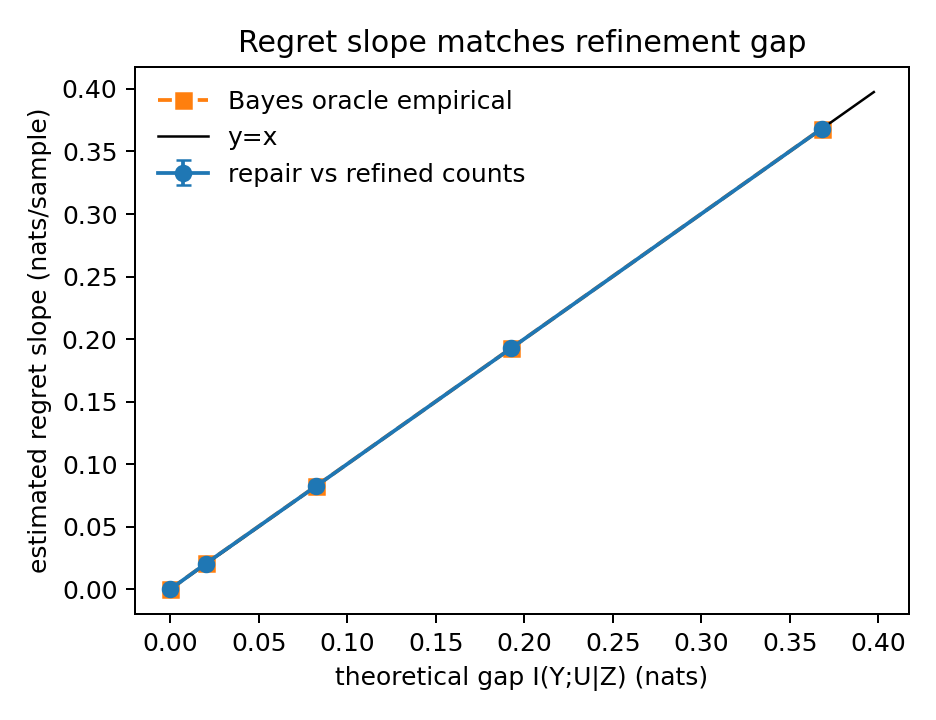
\includegraphics[width=0.62\linewidth]{experiments/refinement_theory_results/bayes_gap_slope_vs_theory.png}
\caption{Known Bayes-gap calibration. The estimated repair-only regret slope matches the theoretical refinement gap $I(Y;U\mid Z)$ under log loss.}
\label{fig:bayes-gap-slope}
\end{figure}

\begin{table}[t]
\centering
\small
\begin{tabular}{ccccc}
\toprule
$\delta$ & Theory gap & Repair/refined slope & Bayes-oracle slope & Accepted noise splits \\
\midrule
$0.0$ & $0.0000$ & $-0.0000\pm0.0000$ & $0.0000\pm0.0000$ & $0.00$ \\
$0.1$ & $0.0201$ & $0.0206\pm0.0013$ & $0.0206\pm0.0013$ & $0.00$ \\
$0.2$ & $0.0823$ & $0.0824\pm0.0012$ & $0.0824\pm0.0012$ & $0.00$ \\
$0.3$ & $0.1927$ & $0.1928\pm0.0041$ & $0.1929\pm0.0041$ & $0.00$ \\
$0.4$ & $0.3681$ & $0.3682\pm0.0037$ & $0.3682\pm0.0038$ & $0.00$ \\
\bottomrule
\end{tabular}
\caption{Regret-slope calibration over 16 seeds. Slopes are in nats per sample, estimated from the second half of each stream. At $\delta=0$, $U$ carries no consequence information and no refinement is accepted.}
\label{tab:bayes-gap-calibration}
\end{table}

The agreement is the important point: the error made by repair-only counts is not an optimizer artifact. Its asymptotic slope is the information-structure gap predicted by the theorem. The $\delta=0$ row is the corresponding negative control.

\subsection{Guarded refine-or-repair decisions}

The second experiment tests whether refinement is consequence-sensitive rather than novelty-sensitive. We create two old atoms. In the repair atom, $Y\sim\mathrm{Bernoulli}(0.8)$ and all candidate distinctions are independent of $Y$, but the current local prediction is deliberately stale at $q(Y=1)=0.2$. The correct action is repair. In the refinement atom, $Y\mid U=0\sim\mathrm{Bernoulli}(0.1)$ and $Y\mid U=1\sim\mathrm{Bernoulli}(0.9)$, so the correct action is to refine by $U$.

The candidate pool contains the true distinction $U$, twenty independent noise bits, and six geometry-only bits that are visually separable but independent of $Y$. Candidate proposal and validation use separate buffers. A refinement is accepted only when its penalized held-out gain exceeds both zero and the held-out repair gain by a margin.

\begin{table}[t]
\centering
\small
\begin{tabular}{ccccc}
\toprule
Scoring buffer & True recall & False refinement & Spurious acceptance & Repair accuracy \\
\midrule
$32$ & $0.956$ & $0.001$ & $0.001$ & $0.999$ \\
$64$ & $0.991$ & $0.000$ & $0.000$ & $1.000$ \\
$128$ & $1.000$ & $0.000$ & $0.000$ & $1.000$ \\
$256$ & $1.000$ & $0.000$ & $0.000$ & $1.000$ \\
$512$ & $1.000$ & $0.000$ & $0.000$ & $1.000$ \\
\bottomrule
\end{tabular}
\caption{Guarded refinement decisions over 800 trials per cell type and buffer size. The learner accepts the consequence-useful distinction and rejects noise or geometry-only distinctions.}
\label{tab:guarded-refinement}
\end{table}

\begin{figure}[t]
\centering
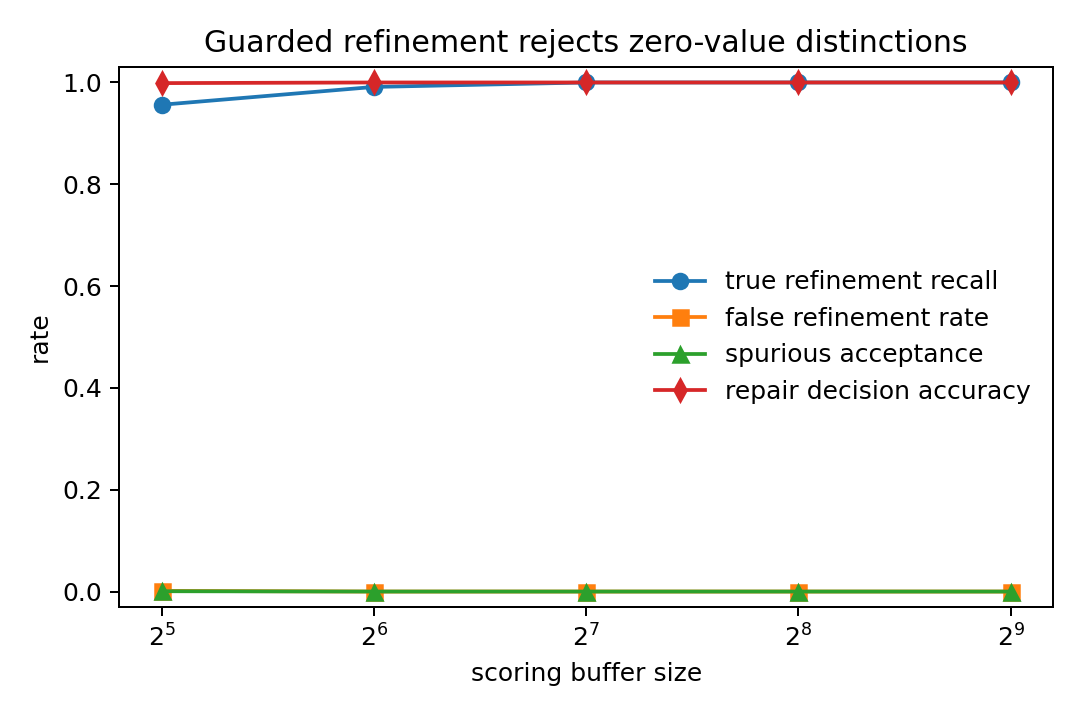
\includegraphics[width=0.62\linewidth]{experiments/refinement_theory_results/guarded_sample_size_curve.png}
\caption{Sample-size curve for the guarded decision rule. Larger scoring buffers preserve true-refinement recall while driving false refinement and spurious acceptance to zero.}
\label{fig:guarded-refinement}
\end{figure}

This directly probes the algorithmic distinction between ``new feature'' and ``useful refinement.'' The repair atom contains a large empirical repair gain and many possible bits, but no bit has stable consequence value, so the guarded rule repairs instead of growing the graph.

\subsection{Graph-memory ablation on contextual XOR}

The third experiment checks the data-structure claim. The stream is a contextual XOR problem: $Y=b_1\oplus b_2\oplus c$, where the initial atoms are keyed by the two visible signs $(b_1,b_2)$ and the useful edge-generated distinction is the context bit $c$. We add nuisance coordinates so that prototype growth and cache baselines can create geometrically distinct states without obtaining the consequence-relevant partition.

\begin{table}[t]
\centering
\scriptsize
\setlength{\tabcolsep}{3pt}
\resizebox{\linewidth}{!}{%
\begin{tabular}{lcccccc}
\toprule
Model & Preq. acc. & Preq. NLL & Test acc. & Concepts & Context edges & Purity \\
\midrule
Full DGM refine+repair+edges & $\mathbf{0.959\pm0.002}$ & $\mathbf{0.073}$ & $\mathbf{0.998}$ & $8.0$ & $4.0$ & $0.997$ \\
DGM repair only & $0.503\pm0.007$ & $0.696$ & $0.502$ & $4.0$ & $0.0$ & $0.514$ \\
DGM refine only, no repair & $0.501\pm0.007$ & $0.693$ & $0.496$ & $8.0$ & $4.0$ & $0.997$ \\
No-edge centroid growth & $0.504\pm0.004$ & $0.698$ & $0.502$ & $8.0$ & -- & $0.155$ \\
$k$NN/cache, same budget & $0.497\pm0.006$ & $0.785$ & $0.499$ & $8.0$ & -- & -- \\
$k$NN/cache, larger budget & $0.494\pm0.005$ & $0.788$ & $0.498$ & $64.0$ & -- & -- \\
\bottomrule
\end{tabular}
}
\caption{Contextual XOR graph-memory ablation over 10 seeds. Full DGM accepts all four context edges and no spurious edges. Repair-only cannot separate incompatible consequences; refine-only recovers the structure but has no local memory repair; no-edge and cache baselines do not recover the consequence partition under the same stream.}
\label{tab:contextual-xor-ablation}
\end{table}

This separates the two mechanisms. Refine-only recovers the right partition structure, as shown by high purity, but without local memory repair its predictions remain at chance. Repair-only has local counts but the wrong atoms. The full graph-memory learner combines edge-generated refinement with local repair and uses only the eight target concepts rather than relying on unbounded growth.

\paragraph{Scope.}
These experiments do not claim that DGM is a finished competitive language-modeling system. They test the mechanisms required by the theory: repair-only regret has the predicted information-structure slope; the refinement rule accepts only consequence-useful distinctions; and graph-generated refinement plus local repair is more effective than either operation alone.

\section{Conclusion}
\label{sec:conclusion}

This paper separates two operations that are often conflated in runtime learning. A repair update improves predictions inside the current information structure. A refinement update changes the information structure itself. The repair-only lower bound shows that, whenever the current quotient collapses cases separated by the target, repair alone incurs linear regret against a refined oracle. The value identities show that useful distinctions are consequence-sensitive: under log loss, their value is conditional mutual information.

DGM realizes these ideas as a graph-memory data structure whose nodes repair local memories and whose edges generate accepted distinctions. The theory does not claim that DGM is a universal replacement for gradient learning. It identifies when fixed-information updates are structurally insufficient and gives one algorithmic mechanism for adding the missing distinctions.

The remaining empirical burden is substantial. The frequency-controlled CIFAR-100 hierarchy query stream shows that the learned graph can recover a real semantic hierarchy in an oracle-partition diagnostic, and the non-oracle CIFAR-100 Image-HQS stream shows that image-routed posterior memory can improve test log loss over online linear and crossed-interaction baselines under a shared frozen encoder. The calibrated trust aggregation gives a cumulative log-loss fallback to the frozen predictor. Stronger nonparametric baselines, memory-latency budgets, larger frozen-embedding streams, and large-scale language-model adaptation remain future work before making broad deployment claims.



\clearpage

\ifdefined\isarxiv
\bibliographystyle{alpha}
\bibliography{ref}
\else
\bibliographystyle{alpha}
\bibliography{ref}
\fi

%%% The part below is the appendix

\newpage
\onecolumn
\appendix

\begin{center}
    \textbf{\LARGE Appendix }
\end{center}

%%% This file is the structure for appendix content
%%% TeX files for body contents should be named as:
%%% 50_xxxx.tex
%%% 51_xxxx.tex
%%% ...

\section{Appendix Roadmap}
\label{app:roadmap}

The appendix follows the same chain as the main text, but with every informal statement replaced by a formal theorem and proof. It first states what the theory does not claim, then places the work relative to existing methods, and then develops the proofs from general projection geometry to exact memory and finally to ridge-statistical memory.
\begin{itemize}
\item {\bf Part 1.} Appendix~\ref{app:limitations} states the limitations of the framework and clarifies which questions remain empirical or architectural rather than settled by the present theory.
\item {\bf Part 2.} Appendix~\ref{app:related} situates Projection Learning among backpropagation, mirror descent, passive-aggressive learning, fast weights, recursive least squares, TTT-style runtime adaptation, and information projection.
\item {\bf Part 3.} Appendix~\ref{app:projection-proofs} proves the general geometry: the Bregman identity, the projection characterization theorem, soft projection inequalities, KL projection, and the relation to implicit and explicit gradient learning.
\item {\bf Part 4.} Appendix~\ref{app:memory-proofs} proves the exact memory story: feasibility, capacity, innovation decomposition, conflict impossibility, conservative hard and soft updates, no-free-repair lower bounds, optimal contraction, and equivalence between sequential hard CPM and batch projection.
\item {\bf Part 5.} Appendix~\ref{app:ridge-proofs} proves the statistical memory story: recursive ridge updates, Bayesian interpretation, normalized competitive prediction, and log-determinant information growth.
\end{itemize}

\section{Limitations}
\label{app:limitations}

The theory identifies when a distinction is necessary or valuable at the population-information level. It does not solve the search problem of finding the best distinction in a rich hypothesis class. The online algorithm is greedy and local: its refinement rule concerns local concepts and their nearby conflicts, not global optimality over all information structures.

The risk identities assume correctly estimated conditional distributions or conditional means. With finite data, refinement can increase estimation error, so useful population distinctions may be statistically unsafe. Complexity penalties, thresholds, validation, Bayesian priors, or minimum leaf sizes are needed in practical systems.

The finite-sample validation theorem assumes a genuinely held-out scoring buffer: fresh samples, or samples not previously used to choose proposals or update the state. Reusing the same validation buffer after previous accept/reject decisions makes the candidate class adaptive to that buffer and requires reusable-holdout or other adaptive-validation machinery beyond the Hoeffding argument stated here.

The base-information convention is restricted. If the full hidden state is made freely conditionable in the Bayes-risk benchmark, then all CA edge predicates and anchor-order events are already measurable and the sigma-algebra refinement gap vanishes. The strict partition theory therefore applies to the current runtime information or to restricted hard-route prediction classes; h-dependent soft memories are implementation approximations or restricted-class extensions.

The graph-growing CA extension specifies one canonical refinement mechanism, based on concepts and local distinction edges, but this is not claimed to be optimal. Rich domains may require learned concept-creation rules, approximate nearest-neighbor indices, nonlinear distinction edges, and better merge, forgetting, or retention-decay policies than the default budget notes in Appendix~\ref{app:dgm-extensions}. The bridge to Projection Memory and CPM is exact for one-hot finite partition memories. Continuous neural representations need additional modeling choices: when a continuous conflict should create a new concept, how local projection memories should be inherited, how retention time scales should be allocated, and how refined information structures interact with differentiable backbones.

CA's dense read avoids sparse candidate-recall assumptions at the concept budgets used in the main experiments, and the current implementation includes fused kernels for the dense concept operations and chunk scan. Large-budget CA will still need sparse concept retrieval, sharded concept banks, and additional fused write/read kernels; at that point candidate recall again becomes an engineering assumption that should be measured in large systems. Edge gates can reject incompatible candidates in the graph-growing extension, but they cannot select a compatible concept that the retrieval layer never exposes.

The large-model layer is an architectural path rather than a completed scaling theorem. It gives a trainable read path, a continuous write path, a trainable retention decay, and a default budget policy with explicit complexity, but it does not prove optimization guarantees for deep nonconvex backbones, nor does it solve distributed systems issues such as load balancing or stale concept shards. The reported fixed-bank implementation now evaluates the exact token-level CA recurrence by chunked affine scan: chunk size affects kernel tiling and parallel depth, not the mathematical causal rule. The remaining systems limitation is efficiency rather than causality: dense CA in every layer is expensive relative to highly optimized Mamba-2/RWKV kernels, so current LM prototypes allocate the dense CoM memory globally and treat layerwise or in-block CoM placements as ablations. The Concept Memory results also show that consequence-feature capacity and the learned decoder are important systems choices: too small a $d_u$ underfits the repaired consequence statistic, while the direct $d_u=d_{\rm model}$ endpoint is not automatically superior in the present residual interface. Budget maintenance in the graph-growing extension is outside the formal refinement theorem: merge, eviction, decay, and compression may discard distinctions, so their effect must be evaluated as a resource-management approximation.

The experiments are a focused sequence-modeling benchmark suite, not a full large-model scaling result. The CoM training probe in Table~\ref{tab:com-training-probe} is a same-stream training-loss comparison, not a final held-out perplexity or downstream zero-shot evaluation. It should be read as evidence for the dense CoM design direction, especially the consequence-sketch capacity result, not as evidence that CA already dominates optimized attention, Mamba, RWKV, GDN, or TTT implementations at production scale. A complete empirical evaluation should include state-equalized MQAR, language modeling at multiple parameter and token budgets, held-out same-corpus PPL, zero-shot task metrics, latency and memory curves, and ablations of chunk size, write-key shift, retention parameterization, consequence-feature dimension, fixed-bank versus dynamic concepts, and edge-free versus edge-gated variants.

\section{Related Work}
\label{app:related}

\paragraph{Prototype and memory methods.} Prototype and memory methods represent data by stored exemplars or centers. DGM uses the same computational intuition but adds a refinement rule: a new prototype is created when local repair cannot absorb evidence without conflating consequences, and distinction edges record the separating evidence.

\paragraph{Decision trees and splitting criteria.} Classical decision trees use information gain and variance reduction as splitting criteria. In our view, a decision tree is a hard-routing special case of a distinction graph. It stores distinctions in a hierarchy rather than as local edges between concepts.

\paragraph{Sparse experts and retrieval layers.} Mixture-of-experts and retrieval-augmented models scale neural computation by selecting a small subset of parameters or memories for each input. A DGM layer has a similar sparse read path, but the selected objects are runtime concepts with local memories, and the write path can refine or repair the state after observing consequences.

\paragraph{Information theory and statistical decision theory.} The log-loss identity is the standard relation between optimal code length and conditional entropy, while the squared-loss identity is the orthogonal decomposition of conditional expectations in $L^2$. Our contribution is to place these identities inside a runtime-learning story: the value of learning a distinction is its reduction in Bayes risk.

\paragraph{Backpropagation and gradient learning.} Backpropagation supplies differentiable credit assignment for fixed computation graphs \citep{rumelhart1986learning}. Distinction Learning addresses a different failure mode: the current information structure may not contain the distinctions needed for any measurable predictor to succeed.

\paragraph{Projection learning and online repair.} Bregman projection, mirror descent, and proximal methods provide minimal-change state updates \citep{bregman1967relaxation,zinkevich2003online,shalev2012online,hazan2016introduction}. Conservative Projection Memory uses this idea for runtime associative repair. The present paper demotes projection repair to the continuous-state layer that operates after the relevant information structure has been fixed.

\paragraph{Test-time adaptation.} Test-time training adapts parameters using auxiliary losses at inference time \citep{sun2020test}. TTT layers treat hidden states as trainable models updated on test sequences \citep{sun2025learning}. Distinction Learning suggests a complementary diagnostic: when runtime evidence conflicts inside an indistinguishable atom, the issue is not only how to update fast state, but what distinction the state failed to represent.

\section{Projection Learning Proofs}
\label{app:projection-proofs}

\begin{lemma}[Bregman three-point identity]
\label{lem:three-point:formal}
For all $a,b,u\in S$,
\begin{align*}
D_\psi(u,a)-D_\psi(u,b)-D_\psi(b,a)=\ip{\nabla\psi(a)-\nabla\psi(b)}{b-u}.
\end{align*}
\end{lemma}
\begin{proof}
Expand each term:
\begin{align*}
D_\psi(u,a)&=\psi(u)-\psi(a)-\ip{\nabla\psi(a)}{u-a},\\
D_\psi(u,b)&=\psi(u)-\psi(b)-\ip{\nabla\psi(b)}{u-b},\\
D_\psi(b,a)&=\psi(b)-\psi(a)-\ip{\nabla\psi(a)}{b-a}.
\end{align*}
Then
\begin{align*}
D_\psi(u,a)-D_\psi(u,b)-D_\psi(b,a)&=-\ip{\nabla\psi(a)}{u-a}+\ip{\nabla\psi(b)}{u-b}+\ip{\nabla\psi(a)}{b-a}\\
&=\ip{\nabla\psi(a)}{b-u}-\ip{\nabla\psi(b)}{b-u}\\
&=\ip{\nabla\psi(a)-\nabla\psi(b)}{b-u}.
\end{align*}
\end{proof}

\begin{theorem}[Projection characterization, formal version of Theorem~\ref{thm:projection-characterization:informal}]
\label{thm:projection-characterization:formal}
Let $S$ be closed and convex, let $\psi$ be differentiable and strictly convex, let $\calC\subseteq S$ be closed and convex, and let $s_0\in S$. For $p\in\calC$, the following are equivalent:
\begin{itemize}
\item {\bf Part 1.} $p=\argmin_{s\in\calC}D_\psi(s,s_0)$.
\item {\bf Part 2.} For all $u\in\calC$,
\begin{align*}
D_\psi(u,p)+D_\psi(p,s_0)\le D_\psi(u,s_0).
\end{align*}
\end{itemize}
\end{theorem}
\begin{proof}
Assume Part 1. The first-order optimality condition is
\begin{align*}
\ip{\nabla\psi(p)-\nabla\psi(s_0)}{u-p}\ge0\qquad \forall u\in\calC.
\end{align*}
Equivalently,
\begin{align*}
\ip{\nabla\psi(s_0)-\nabla\psi(p)}{p-u}\ge0\qquad \forall u\in\calC.
\end{align*}
By Lemma~\ref{lem:three-point:formal},
\begin{align*}
D_\psi(u,s_0)-D_\psi(u,p)-D_\psi(p,s_0)=\ip{\nabla\psi(s_0)-\nabla\psi(p)}{p-u}.
\end{align*}
Thus Part 2 follows.

Assume Part 2. The same identity implies
\begin{align*}
\ip{\nabla\psi(s_0)-\nabla\psi(p)}{p-u}\ge0\qquad \forall u\in\calC.
\end{align*}
Hence
\begin{align*}
\ip{\nabla\psi(p)-\nabla\psi(s_0)}{u-p}\ge0\qquad \forall u\in\calC.
\end{align*}
This is the variational inequality for minimizing $D_\psi(s,s_0)$ over $\calC$. Strict convexity gives uniqueness, so Part 1 follows.
\end{proof}

\begin{corollary}[Fejer monotonicity and bounded drift]
\label{cor:fejer:formal}
Let $s_{t+1}=\argmin_{s\in\calC_t}D_\psi(s,s_t)$. If $u^\star\in\cap_{t=1}^T\calC_t$, then
\begin{align*}
D_\psi(u^\star,s_{t+1})\le D_\psi(u^\star,s_t)
\end{align*}
and
\begin{align*}
\sum_{t=1}^T D_\psi(s_{t+1},s_t)\le D_\psi(u^\star,s_1).
\end{align*}
\end{corollary}
\begin{proof}
By Theorem~\ref{thm:projection-characterization:formal},
\begin{align*}
D_\psi(u^\star,s_{t+1})+D_\psi(s_{t+1},s_t)\le D_\psi(u^\star,s_t).
\end{align*}
Dropping the second term gives the first claim. Summing gives
\begin{align*}
\sum_{t=1}^T D_\psi(s_{t+1},s_t)&\le \sum_{t=1}^T\left(D_\psi(u^\star,s_t)-D_\psi(u^\star,s_{t+1})\right)\\
&=D_\psi(u^\star,s_1)-D_\psi(u^\star,s_{T+1})\\
&\le D_\psi(u^\star,s_1).
\end{align*}
\end{proof}

\begin{theorem}[Soft projection inequality]
\label{thm:soft-projection:formal}
Let $\ell_t:S\to\R$ be convex and let
\begin{align*}
s_{t+1}=\argmin_{s\in S}\{D_\psi(s,s_t)+\eta_t\ell_t(s)\}.
\end{align*}
Then for all $u\in S$,
\begin{align*}
\eta_t(\ell_t(s_{t+1})-\ell_t(u))\le D_\psi(u,s_t)-D_\psi(u,s_{t+1})-D_\psi(s_{t+1},s_t).
\end{align*}
\end{theorem}
\begin{proof}
For some $g_{t+1}\in\partial\ell_t(s_{t+1})$, optimality gives
\begin{align*}
\ip{\nabla\psi(s_{t+1})-\nabla\psi(s_t)+\eta_t g_{t+1}}{u-s_{t+1}}\ge0.
\end{align*}
Thus
\begin{align*}
\eta_t\ip{g_{t+1}}{s_{t+1}-u}\le \ip{\nabla\psi(s_t)-\nabla\psi(s_{t+1})}{s_{t+1}-u}.
\end{align*}
Convexity gives
\begin{align*}
\ell_t(s_{t+1})-\ell_t(u)\le \ip{g_{t+1}}{s_{t+1}-u}.
\end{align*}
Lemma~\ref{lem:three-point:formal} gives
\begin{align*}
\ip{\nabla\psi(s_t)-\nabla\psi(s_{t+1})}{s_{t+1}-u}=D_\psi(u,s_t)-D_\psi(u,s_{t+1})-D_\psi(s_{t+1},s_t).
\end{align*}
Combining proves the claim.
\end{proof}

\begin{theorem}[KL consistency projection]
\label{thm:kl-projection:formal}
Let $p_t$ be strictly positive on a finite space $\calX$. The solution of
\begin{align*}
\argmin_{p:\mathbb E_p[\phi]=c}D_{\mathrm{KL}}(p\|p_t)
\end{align*}
has the form
\begin{align*}
p_{t+1}(x)=\frac{p_t(x)\exp(\lambda^\top\phi(x))}{Z(\lambda)}.
\end{align*}
\end{theorem}
\begin{proof}
The Lagrangian is
\begin{align*}
\calL(p,\lambda,\nu)=\sum_x p(x)\log\frac{p(x)}{p_t(x)}+\lambda^\top\left(\sum_x p(x)\phi(x)-c\right)+\nu\left(\sum_xp(x)-1\right).
\end{align*}
Stationarity gives
\begin{align*}
\log\frac{p(x)}{p_t(x)}+1+\lambda^\top\phi(x)+\nu=0.
\end{align*}
Hence, after absorbing signs into $\lambda$ and normalizing,
\begin{align*}
p_{t+1}(x)=\frac{p_t(x)\exp(\lambda^\top\phi(x))}{Z(\lambda)}.
\end{align*}
\end{proof}

\begin{proposition}[Gradient descent as linearized projection]
\label{prop:gd-linearized:formal}
For $D_\psi(s,s_t)=\norm{s-s_t}_2^2/2$, replacing $\ell_t(s)$ in the soft projection objective by its first-order approximation at $s_t$ gives $s_{t+1}=s_t-\eta\nabla\ell_t(s_t)$.
\end{proposition}
\begin{proof}
The linearized objective is
\begin{align*}
\frac{1}{2}\norm{s-s_t}^2+\eta\ip{\nabla\ell_t(s_t)}{s-s_t}+\eta\ell_t(s_t).
\end{align*}
The stationarity condition is
\begin{align*}
s-s_t+\eta\nabla\ell_t(s_t)=0.
\end{align*}
Thus
\begin{align*}
s_{t+1}=s_t-\eta\nabla\ell_t(s_t).
\end{align*}
\end{proof}

\section{Conservative Memory Proofs}
\label{app:memory-proofs}

\begin{theorem}[Exact associative binding, formal version of Theorem~\ref{thm:exact-binding:informal}]
\label{thm:exact-binding:formal}
Let $K\in\R^{r\times T}$ and $V\in\R^{m\times T}$. The set $\calC=\{W\in\R^{m\times r}:WK=V\}$ is nonempty if and only if $\ker K\subseteq\ker V$. If $\calC$ is nonempty, then
\begin{align*}
\argmin_{W\in\calC}\frac{1}{2}\norm{W-W_0}_F^2=W_0+(V-W_0K)K^+.
\end{align*}
\end{theorem}
\begin{proof}
If $WK=V$ and $a\in\ker K$, then
\begin{align*}
Va=WKa=0.
\end{align*}
Thus $\ker K\subseteq\ker V$.

Assume $\ker K\subseteq\ker V$. Since $K^+K$ is the orthogonal projector onto $(\ker K)^\perp$, the condition implies
\begin{align*}
V=VK^+K.
\end{align*}
Thus $W=VK^+$ satisfies $WK=V$.

Let $R=V-W_0K$ and $W=W_0+\Delta$. The projection problem is
\begin{align*}
\min_\Delta\frac{1}{2}\norm{\Delta}_F^2\quad \text{subject to}\quad \Delta K=R.
\end{align*}
The minimum-norm solution is
\begin{align*}
\Delta^\star=RK^+.
\end{align*}
Therefore
\begin{align*}
W^\star=W_0+(V-W_0K)K^+.
\end{align*}
\end{proof}

\begin{theorem}[Innovation decomposition, formal version of Theorem~\ref{thm:innovation-decomposition:informal}]
\label{thm:innovation-decomposition:formal}
Assume $WK=V$. Let $\Pi=KK^+$, $z=(I-\Pi)k$, and $a=K^+k$. Then
\begin{align*}
Wk=Va+Wz.
\end{align*}
If $z=0$, $Wk$ is fixed over all old-feasible $W$. If $z\ne0$, the constraint $Wk=v$ is equivalent over old-feasible $W$ to $Wz=v-Va$.
\end{theorem}
\begin{proof}
The decomposition is
\begin{align*}
k=KK^+k+(I-KK^+)k=Ka+z.
\end{align*}
Multiplying by $W$ gives
\begin{align*}
Wk=WKa+Wz=Va+Wz.
\end{align*}
If $z=0$, then $Wk=Va$ for every $W$ satisfying $WK=V$. If $z\ne0$, then
\begin{align*}
Wk=v\quad \Longleftrightarrow\quad Va+Wz=v\quad \Longleftrightarrow\quad Wz=v-Va.
\end{align*}
\end{proof}

\begin{theorem}[Conflict impossibility, formal version of Theorem~\ref{thm:conflict-impossibility:informal}]
\label{thm:conflict-impossibility:formal}
Assume $W_tK=V$ and $z=(I-KK^+)k=0$. If $W_t+\Delta$ preserves old evidence, then $(W_t+\Delta)k=W_tk$. Hence $Wk=v$ is compatible with old evidence if and only if $v=W_tk$.
\end{theorem}
\begin{proof}
Preserving old evidence means
\begin{align*}
(W_t+\Delta)K=V=W_tK.
\end{align*}
Thus
\begin{align*}
\Delta K=0.
\end{align*}
If $z=0$, then $k\in\Span(K)$, hence
\begin{align*}
\Delta k=0.
\end{align*}
Therefore
\begin{align*}
(W_t+\Delta)k=W_tk.
\end{align*}
\end{proof}

\begin{theorem}[Hard Conservative Projection Memory]
\label{thm:hard-cpm:formal}
Assume $W_tK=V$, let $\Pi=KK^+$, $z=(I-\Pi)k\ne0$, and $e=v-W_tk$. Then
\begin{align*}
W_{t+1}=W_t+\frac{ez^\top}{\norm{z}^2}
\end{align*}
preserves $WK=V$, satisfies $Wk=v$, and minimizes $\norm{W-W_t}_F^2/2$ among all memories satisfying both constraints.
\end{theorem}
\begin{proof}
Let $\Delta^\star=ez^\top/\norm{z}^2$. Since $z\perp\Span(K)$,
\begin{align*}
\Delta^\star K=0.
\end{align*}
Thus
\begin{align*}
W_{t+1}K=W_tK=V.
\end{align*}
Also $z^\top k=\norm{z}^2$, so
\begin{align*}
\Delta^\star k=e.
\end{align*}
Hence
\begin{align*}
W_{t+1}k=W_tk+e=v.
\end{align*}
For minimality, any feasible update $\Delta$ satisfies
\begin{align*}
\Delta K=0,\qquad \Delta k=e.
\end{align*}
Since $\Delta K=0$,
\begin{align*}
\Delta k=\Delta(I-\Pi)k=\Delta z.
\end{align*}
Thus the problem reduces to
\begin{align*}
\min_\Delta\frac{1}{2}\norm{\Delta}_F^2\quad \text{subject to}\quad \Delta z=e.
\end{align*}
The minimum-norm solution is $\Delta^\star=ez^\top/\norm{z}^2$.
\end{proof}

\begin{theorem}[Soft Conservative Projection Memory, formal version of Theorem~\ref{thm:soft-cpm:informal}]
\label{thm:soft-cpm:formal}
Assume $W_tK=V$, let $\Pi=KK^+$, $z=(I-\Pi)k\ne0$, and $e=v-W_tk$. The unique solution of
\begin{align*}
\argmin_{W:WK=V}\left\{\frac{1}{2}\norm{W-W_t}_F^2+\frac{\eta}{2}\norm{Wk-v}^2\right\}
\end{align*}
is
\begin{align*}
W_{t+1}=W_t+\frac{\eta}{1+\eta\norm{z}^2}ez^\top.
\end{align*}
Moreover,
\begin{align*}
W_{t+1}K=V,\qquad v-W_{t+1}k=\frac{1}{1+\eta\norm{z}^2}e.
\end{align*}
\end{theorem}
\begin{proof}
Write $W=W_t+\Delta$. The constraint $WK=V$ is equivalent to
\begin{align*}
\Delta K=0.
\end{align*}
Since $\Delta K=0$,
\begin{align*}
\Delta k=\Delta(I-\Pi)k=\Delta z.
\end{align*}
The objective becomes
\begin{align*}
\min_{\Delta:\Delta K=0}\frac{1}{2}\norm{\Delta}_F^2+\frac{\eta}{2}\norm{\Delta z-e}^2.
\end{align*}
The stationarity equation in the feasible subspace is
\begin{align*}
\Delta+\eta(\Delta z-e)z^\top=0.
\end{align*}
Let $\Delta=\alpha ez^\top$. Substitution gives
\begin{align*}
\alpha ez^\top+\eta(\alpha e\norm{z}^2-e)z^\top=0.
\end{align*}
Thus
\begin{align*}
\alpha(1+\eta\norm{z}^2)=\eta.
\end{align*}
Therefore
\begin{align*}
\Delta=\frac{\eta}{1+\eta\norm{z}^2}ez^\top.
\end{align*}
Since $z^\top K=0$, $W_{t+1}K=V$. The residual is
\begin{align*}
v-W_{t+1}k&=e-\Delta k\\
&=e-\Delta z\\
&=e-\frac{\eta\norm{z}^2}{1+\eta\norm{z}^2}e\\
&=\frac{1}{1+\eta\norm{z}^2}e.
\end{align*}
\end{proof}

\section{Ridge and Bayesian Projection Memory Proofs}
\label{app:ridge-proofs}

\begin{theorem}[Ridge solution]
\label{thm:ridge-solution:formal}
Let
\begin{align*}
J_t(W)=\frac{\lambda}{2}\norm{W-W_0}_F^2+\frac{1}{2}\sum_{\tau=1}^t\rho_\tau\norm{Wk_\tau-v_\tau}^2.
\end{align*}
Define
\begin{align*}
A_t=\lambda I+\sum_{\tau=1}^t\rho_\tau k_\tau k_\tau^\top,\qquad B_t=\lambda W_0+\sum_{\tau=1}^t\rho_\tau v_\tau k_\tau^\top.
\end{align*}
Then the unique minimizer is $W_{t+1}=B_tA_t^{-1}$.
\end{theorem}
\begin{proof}
Differentiate:
\begin{align*}
\nabla J_t(W)=\lambda(W-W_0)+\sum_{\tau=1}^t\rho_\tau(Wk_\tau-v_\tau)k_\tau^\top.
\end{align*}
At optimum,
\begin{align*}
0=\lambda(W-W_0)+\sum_{\tau=1}^t\rho_\tau(Wk_\tau-v_\tau)k_\tau^\top.
\end{align*}
Thus
\begin{align*}
W\left(\lambda I+\sum_{\tau=1}^t\rho_\tau k_\tau k_\tau^\top\right)=\lambda W_0+\sum_{\tau=1}^t\rho_\tau v_\tau k_\tau^\top.
\end{align*}
Since $\lambda>0$, $A_t$ is invertible. Hence
\begin{align*}
W_{t+1}=B_tA_t^{-1}.
\end{align*}
\end{proof}

\begin{theorem}[Recursive ridge update]
\label{thm:ridge-recursive:formal}
Let $P_t=A_{t-1}^{-1}$ and $W_t=B_{t-1}P_t$. Define
\begin{align*}
g_t=\frac{\rho_tP_tk_t}{1+\rho_t k_t^\top P_tk_t}.
\end{align*}
Then
\begin{align*}
W_{t+1}=W_t+(v_t-W_tk_t)g_t^\top,\qquad P_{t+1}=P_t-\frac{\rho_tP_tk_tk_t^\top P_t}{1+\rho_t k_t^\top P_tk_t}.
\end{align*}
\end{theorem}
\begin{proof}
The Sherman-Morrison identity gives
\begin{align*}
P_{t+1}=A_t^{-1}=P_t-\frac{\rho_tP_tk_tk_t^\top P_t}{1+\rho_t k_t^\top P_tk_t}.
\end{align*}
Let $a_t=k_t^\top P_tk_t$. Then
\begin{align*}
k_t^\top P_{t+1}=k_t^\top P_t-\frac{\rho_ta_t k_t^\top P_t}{1+\rho_ta_t}=\frac{k_t^\top P_t}{1+\rho_ta_t}.
\end{align*}
Using $B_t=B_{t-1}+\rho_tv_tk_t^\top$,
\begin{align*}
W_{t+1}&=B_tP_{t+1}\\
&=B_{t-1}P_{t+1}+\rho_tv_tk_t^\top P_{t+1}\\
&=W_t-\frac{\rho_tW_tk_tk_t^\top P_t}{1+\rho_ta_t}+\frac{\rho_tv_tk_t^\top P_t}{1+\rho_ta_t}\\
&=W_t+(v_t-W_tk_t)\frac{\rho_tk_t^\top P_t}{1+\rho_ta_t}\\
&=W_t+(v_t-W_tk_t)g_t^\top.
\end{align*}
\end{proof}

\begin{theorem}[Bayesian ridge projection memory, formal version of Theorem~\ref{thm:bayesian-ridge:informal}]
\label{thm:bayesian-ridge:formal}
Assume each row $w_j$ of $W$ has prior $w_j\sim\mathcal N(w_{0,j},\lambda^{-1}I)$ and observations satisfy $v_t=Wk_t+\varepsilon_t$ with $\varepsilon_t\sim\mathcal N(0,\rho_t^{-1}I_m)$ independently over time. Then the posterior mean and MAP estimate are $B_tA_t^{-1}$.
\end{theorem}
\begin{proof}
The negative log posterior, up to constants independent of $W$, is
\begin{align*}
\frac{\lambda}{2}\norm{W-W_0}_F^2+\frac{1}{2}\sum_{\tau=1}^t\rho_\tau\norm{Wk_\tau-v_\tau}^2.
\end{align*}
This is $J_t(W)$. The posterior is Gaussian because the prior is Gaussian and the observation model is linear Gaussian. Hence the posterior mean equals the MAP. By Theorem~\ref{thm:ridge-solution:formal}, this value is
\begin{align*}
B_tA_t^{-1}.
\end{align*}
\end{proof}



\ifdefined\isarxiv
\else
\newpage
\section*{NeurIPS Paper Checklist}

This file is retained only for the conference-template branch of \texttt{main.tex}. The current draft is configured as an arXiv-style theoretical paper via \texttt{\textbackslash def\textbackslash isarxiv\{1\}} in \texttt{\_0\_vars.tex}, so this checklist is not included in the compiled manuscript.

\begin{itemize}
\item {\bf Claims.} The abstract and introduction state the paper's scope as a theoretical and architectural proposal: runtime learning by minimal consistency repair, instantiated as Conservative Projection Memory.
\item {\bf Limitations.} Appendix~\ref{app:limitations} states the main limitations, including evidence quality, nonstationarity, approximate innovation maintenance, and lack of empirical claims.
\item {\bf Theory assumptions and proofs.} The assumptions appear in the theorem statements in Sections~\ref{sec:preliminaries}--\ref{sec:main-results}; full proofs are in Appendices~\ref{app:projection-proofs}--\ref{app:ridge-proofs}.
\item {\bf Experiments.} The draft is a theoretical paper and does not report empirical results.
\end{itemize}

\fi

\end{document}
